\documentclass[twoside]{scrartcl}

\usepackage[blacklinks]{drangreport}
% \usepackage[caecilia]{drangreport}

\usepackage{pgfplots}

%Thomas' contradiction symbol
\newcommand*{\cont}{%
  \mathsf{X}\mkern-8.5mu\mathsf{X}%
}
\renewcommand{\thempfootnote}{$\dagger$}

%Change font of proof to scshape, not sure if it looks better...
\expandafter\let\expandafter\oldproof\csname\string\proof\endcsname
\let\oldendproof\endproof
\renewenvironment{proof}[1][\proofname]{%
  \oldproof[\scshape #1]%
}{\oldendproof}


\title{Analysis I}


\hypersetup{pdfinfo={
Title={Analysis I},
Author={Karim Bacchus},
Keywords ={Analysis I, M1P1, Lecture Notes, Imperial College, Maths},
}}


\begin{document}


\NotesTitle{1st}{Spring 2015}{Analysis I}{Prof.~R.}{Thomas}
{
Caveat Lector: unofficial notes, \emph{not} endorsed by Imperial College.\\[0.1cm]
Comments and corrections should be sent to \href{mailto:kb514@ic.ac.uk}{\texttt{kb514@ic.ac.uk}}
}
{

\section*{About these notes}

These notes are not affiliated with Richard Thomas (or even \emph{Professor} Richard Thomas!)\\ The \LaTeX{} source is available on \texttt{github} - it would be great if someone would update changes to the courses so they'll still be useful to later years. Notes for other courses are available on \texttt{dropbox}:

\begin{center}
\begin{tabular}{l | l}
\textbf{1st / 2nd Year} & \textbf{3rd / 4th Year}\\
Foundations of Analysis & Galois Theory\\
Analysis I & Algebraic Number Theory \\
Analysis II & Analytical Number Theory \\
Complex Analysis & Elliptic Curves  \\
Geometry \& Linear Algebra & Modular Forms \\
Algebra I & Algebra III \\
Algebra II & Commutative Algebra \\
Methods I & Lie Algebras  \\
Methods II & Measure \& Integration  \\
Multivariable Calculus & Functional Analysis\\
Differential Equations & Algebraic Topology \\
Metric Spaces \& Topology  & Differential Topology \\
Intro to Numerical Analysis & Complexity \\
Mechanics & General Relativity \\
\end{tabular}
\end{center}

\begin{flushright}
- Karim Bacchus 	
\end{flushright}



\pagebreak 
\thispagestyle{empty}


\section*{Syllabus}  

\textit{A rigorous treatment of the concept of a limit, as applied to sequences, series and functions.}
\begin{itemize}
\item  Real and complex sequences. Convergence, divergence and divergence to infinity. Sums and products of convergent sequences. The Sandwich Test. Sub-sequences, monotonic sequences, Bolzano-Weierstrass Theorem. Cauchy sequences and the general principle of convergence.

\item Real and complex series. Convergent and absolutely convergent series. The Comparison Test for non-negative series and for absolutely convergent series. The Alternating Series Test.  Rearranging absolutely convergent series. Radius of convergence of power series. The exponential series.

\item Limits and continuity of real and complex functions. Left and right limits and continuity. Maxima
and minima of real valued continuous functions on a closed interval. Inverse Function Theorem for
strictly monotonic real functions on an interval. 

\item  An introduction to differentiability: definitions, examples, left and right derivative.
\end{itemize}
\subsection*{Appropriate books}

{\shortskip

K.~G.~ Binmore, \textit{Mathematical Analysis, A Straightforward Approach} (Cambridge University Press).

}

}





\TableofContents
\stepcounter{lecture}

\pagebreak
\setcounter{section}{-1}

\setcounter{lecture}{0}

\sektion{Preliminaries}
\lecturemarker{1}{5 Oct}


M1F stuff:

\begin{itemize}
\item $\forall - \text{ for any, \textbf{fix any}, for all, every...}$
\item $\exists - \text{ there exists}$
\item $\mathbb{N} = \{1,2,3,\dots\}$ 
\end{itemize}

\begin{theorem}[Triangle Inequality]
(See Question Sheet 1)
	\[|a+b| \leq |a| + |b|\]
\end{theorem}

\begin{corollary}
\[\left||a| - |b|\right|\leq |a-b|	\]
\end{corollary}
\begin{proof}
\[
\begin{aligned}
|a-b| < \epsilon &\iff b-\epsilon < a < b + \epsilon\\
&\iff a \in (b-\epsilon, b+\epsilon)\\
&\iff b \in (a-\epsilon, a+\epsilon)	\\
&\implies \left||a| - |b|\right|< \epsilon
\end{aligned} \] 
\end{proof}

Lots of other versions, see Question Sheet 1 - \emph{don't try to memorise them!}\\



\begin{clicker}
Fix $a \in \mathbb{R}$. What does the statement 
\[\forall \epsilon >0,~|x-a|<\epsilon ~(*)\]
mean for the number $x$? 

\textbf{Answer:} $x = a$. 
\begin{proof}
Assume $x \neq a$. Take $\epsilon := \frac{1}{2}|x-a| > 0$. Then $(*)$ does not hold.	
\end{proof}

\end{clicker}







\stepcounter{lecture}
\setcounter{lecture}{1}

\sektion{Sequences}
\lecturemarker{2}{5 Oct}
\label{sub:sequences}

A sequence $(a_n)_{n\geq 1}$ of real (or complex, etc.) numbers is an infinite list of numbers $a_1,~a_2,~a_3,\dots$ all in $\mathbb{R}$ (or $\mathbb{C}$, etc.) Formally:\\

\begin{definition}
	A \emph{sequence} is a function $a:\mathbb{N} \to \mathbb{R}$
\end{definition}

\textbf{Notation:} We let $a_n \in \mathbb{R}$ denote $a(n)$ for $n \in \mathbb{N}$. The data $(a_n)_{n=1,2,\dots}$ is equivalent to the function $a:\mathbb{N} \to \mathbb{R}$ because a function $a$ is determined by its values $a_n$ over all $n \in \mathbb{N}$. 

We will denote $a$ by $a_1,~a_2,\dots$ or $(a_n)_{n\in\mathbb{N}}$ or $(a_n)_{n\geq 1}$ or even just $(a_n)$.

\begin{remark}
$a_i$'s could be repeated, so $(a_n)$ is \emph{not} equivalent to the set $\{a_n : n \in \mathbb{N}\}\subset \mathbb{R}$. E.g. $(a_n) = 1,~0,~1,~0,\dots$ is different from $(b_n) = 1,~0,~0,~1,~0,~0,~1,\dots$	
\end{remark}

We can describe a sequence in may ways, e.g. formula for $a_n$ as above $a_n = \frac{1-(-1)^n}{2}$, or a recursion e.g. $c_1 = 1 = c_2$, $c_n = c_{n-1} + c_{n-2}$ for $n\geq 3$, or a summation (see next section) e.g. $d_n = \sum_{i=1}^n \frac{1}{i} = 1 + \frac{1}{2} + \frac{1}{3} + \dots +\frac{1}{n}$.

\subsektion{Convergence of Sequences}
We want to \emph{rigorously} define $a_n \to a \in \mathbb{R}$, or ``$a_n$ converges to $a$ as $n \to \infty$" or ``$a$ is the limit of $(a_n)$". 

Idea: $a_n$ should get closer and closer to $a$. Not necessarily monotonically, e.g.:
\[a_n = 
\begin{cases}
\frac{1}{n} & n \text{ odd}\\
\frac{1}{2n} & n \text{ even}	
\end{cases}
\hspace*{20pt}\text{ we want } a_n \to 0\]


\begin{center}
\begin{tikzpicture}
\begin{axis}[axis lines=middle,
     x label style={at={(axis description cs:0.95,-0.15)}},
     y label style={at={(axis description cs:-0.1,0.9)}},
    xlabel={$n$},
    ylabel={$a_n$},
    ticks=none,
  ymin = 0,
  ymax = 0.4,
  xmin = 1,
  xmax = 10,
  width=10cm,height=5cm]
   \addplot[samples at={3,5,7,9}, only marks, mark=x, mark size=3pt]{1/x};
    \addplot[samples at={2,4,6,8},only marks,mark=x,mark size=3pt]{(1/(2*x))};
  \end{axis}
\end{tikzpicture}
\end{center}
Also notice that $\frac{1}{n}$ gets closer and closer to $-1$! So we want to say instead that $a_n$ gets \emph{as close as we like to $a$}. We will measure this with $\epsilon >0$. We phrase ``$a_n$ gets \emph{arbitrarily} close to $a$" by ``$a_n$ gets to within $\epsilon$ of $a$ for \emph{any} $\epsilon >0$".\\

\begin{definition}[Mestel]
	$u_n \to u$ if $\forall n$ sufficiently large, $|u_n - u|$ is \emph{arbitrarily small.} 
	
Define a real number $b \in \mathbb{R}$ to be arbitrarily small if it is smaller than any $\epsilon >0$ i.e. $\forall \epsilon >0,~|b| < \epsilon$.
\end{definition}

Definition Mestel says that once $n$ is large enough, $|u_n - u|$ is less than every $\epsilon >0$, i..e it's zero, i.e. $u_n = u$. We want to \emph{reverse} the order of specifying $n$ and $\epsilon$. 

i.e. we want to say that to get \emph{arbitrarily close to the limit $a$} (i.e. $|a_n - a| < \epsilon$), we need to go sufficiently far down the sequence. Then if I change $\epsilon >0$ to be smaller, I simply go further down the sequence to get within $\epsilon$ of $a$. \\



\begin{center}
\begin{tikzpicture}
\begin{axis}[
 axis line style={red},
axis lines=middle,
     x label style={at={(axis description cs:1.05,0.33)}},
     y label style={at={(axis description cs:-0.1,1.1)}},
    xlabel={\small $n$},
    ylabel={$a_n \to 0$},
  ymin = -0.4,
  ymax = 0.7,
  xmin = 1,
  xmax = 20,
    ytick = {0.3,0.12},
   yticklabels={$\epsilon_1$,$\epsilon_2$},
   xtick = 0,
  width=12cm,height=8cm]
   \addplot[samples at={2,...,20}, only marks, mark=x, mark size=2pt,  mark options={red},]{1/x};
   \draw (axis cs:20,0.3) -- (axis cs:0,0.3);
      \draw (axis cs:20,0.12) -- (axis cs:0,0.12);
     \draw (axis cs:20,-.1) -- (axis cs:4,-.1) node at (axis cs:10,-0.15){\small $n$ suff. large for $|a_n - 0| < \epsilon_1$};
          \draw (axis cs:4,-.06) -- (axis cs:4,-.1);
          \draw (axis cs:20,-.06) -- (axis cs:20,-.1);
          \draw (axis cs:20,-.25) -- (axis cs:9,-.25) node at (axis cs:15,-0.3){\small $n$ suff. large for $|a_n - 0| < \epsilon_2$};
           \draw (axis cs:9,-.2) -- (axis cs:9,-.25);
          \draw (axis cs:20,-.2) -- (axis cs:20,-.25);

  \end{axis}
\end{tikzpicture}
\end{center}

There will not be a ``$n$ sufficiently large" that works for all $\epsilon$ at once! (unless $a_n = a$ eventually.)

But for \emph{any} (fixed) $\epsilon>0$ we want there to be an $n$ sufficiently large such that $|a_n - a| < \epsilon$. So we change ``$\exists n$ such that $\forall \epsilon$" to ``$\forall \epsilon,~\exists n.$". \emph{This allows $n$ to depend on $\epsilon$.}~\\

\begin{definition}[Nestel]
	$a_n \to a$ if $\forall \epsilon >0,~\exists n \in \mathbb{N}$ such that $|a_n - a| < \epsilon$. 
\end{definition}

e.g. 
\[
a_n = \begin{cases}
 0 & n\text{ even}\\
 1 & n\text{ odd}	
 \end{cases}
 \text{ satisfies } a_n \to 0 \text{ according to Prof. Nestel.}
\]

We want to modify this to say eventually $|a_n - a| < \epsilon$ \emph{and it stays there!}\\

\lecturemarker{3}{5 Oct}

\begin{definition}[Actual Convergence]
We say that $a_n \to a$ iff 
\[\forall \epsilon >0,~\exists N \in \mathbb{N} \text{ such that } ``n \geq N \implies |a_n - a| < \epsilon"\]	
\end{definition}

This says that \emph{however close} ($\forall \epsilon>0$) I want to get to the limit $a$, there's a point in the sequence ($\exists N \in \mathbb{N}$) beyond which ($n \geq N$) my $a_n$ is indeed that close to the limit $a$ ($|a_n - a| <\epsilon$).\\ 

\begin{remark}
$N$ depends on $\epsilon$! $N = N(\epsilon)$	
\end{remark}

Equivalently:
\[\forall \epsilon >0,~ \exists N \in \mathbb{N} \text{ such that} ``\forall n \geq N,~|a_n -a|<\epsilon"\]
or equivalently
\[\forall \epsilon >0,~\exists N_\epsilon\in\mathbb{N} \text{ such that } |a_n - a| < \epsilon,~\forall n \geq N_\epsilon\]

\begin{clicker}Given a sequence of real numbers $(a_n)_{n\geq 1}$. Conisder 
\[\boxed{\forall n \geq 1,~\exists \epsilon >0 \text{ such that } |a_n|< \epsilon}\]
This means? 

\textbf{Answer:} It always holds. \begin{proof}
 Fix any $n \in \mathbb{N}$. Take $\epsilon = |a_n| + 1$. 	
 \end{proof}
 
What about
 \[\boxed{\exists \epsilon >0 \text{ such that } \forall n \geq 1,~|a_n| < \epsilon} \]
 
 \textbf{Answer:} $(a_n)$ is bounded.
 
 
\begin{center}
\begin{tikzpicture}
\begin{axis}[
 axis line style={red},
axis lines=middle,
     x label style={at={(axis description cs:1.05,0.4)}},
     y label style={at={(axis description cs:-0.1,1.1)}},
    xlabel={\small $n$},
    ylabel={$a_n$},
  ymin = -0.4,
  ymax = 0.4,
  xmin = 1,
  xmax = 10,
     ytick = {0.3, -.3},
   yticklabels={$\epsilon$,$-\epsilon$},
   xtick = 0,
  width=10cm,height=5cm]
   \addplot[samples at={5,7,9}, only marks, mark=x,  mark options={red}, mark size=3pt]{(-1)^x*1/x};
    \addplot[samples at={2,3,4,6,8},only marks, mark options={red},mark=x,mark size=3pt]{(1/(2*x))};
       \draw (axis cs:20,0.3) -- (axis cs:0,0.3);
      \draw (axis cs:20,-0.3) -- (axis cs:0,-0.3);
  \end{axis}
\end{tikzpicture}
\end{center}


  \begin{proof}
$\iff a_n \in (-\epsilon,\epsilon)~ \forall n \iff |a_n|$ is bounded by $\epsilon$. \end{proof}

\end{clicker}~

\begin{definition}
If $a_n$ does not converge to $a$ for any $a\in \mathbb{R}$, we say that $a_n$ \emph{diverges.}
\end{definition}~

\begin{example}
I claim that $\frac{1}{n} \to 0$ as $n \to \infty$

\textit{Rough working:} Fix $\epsilon >0$. I want to find $N \in \mathbb{N}$ such that $|a_n - a| = |\frac{1}{n} - 0| = \frac{1}{n} < \epsilon$ for all $n \geq N$. 
\begin{center}
\begin{tikzpicture}
\begin{axis}[
 axis line style={red},
axis lines=middle,
     x label style={at={(axis description cs:1.05,0.1)}},
     y label style={at={(axis description cs:-0.1,1.1)}},
    xlabel={\small $n$},
    ylabel={$a_n$},
  ymin = -0.1,
  ymax = 0.4,
  xmin = 1,
  xmax = 10,
     ytick = {0.15},
   yticklabels={$\epsilon$},
   xtick = 0,
  width=10cm,height=5cm]
   \addplot[samples at={5,7,9}, only marks, mark=x,  mark options={red}, mark size=3pt]{(-1)^x*1/x};
    \addplot[samples at={2,3,4,6,8},only marks, mark options={red},mark=x,mark size=3pt]{(1/(2*x))};
       \draw (axis cs:20,0.15) -- (axis cs:0,0.15);
        \draw (axis cs:4,0.12) -- (axis cs:4,-0.1) node at (axis cs:4.2,-0.05) {$N$};
  \end{axis}
\end{tikzpicture}
\end{center}


Since $a_n = \frac{1}{n}$ is monotonic, it is \emph{sufficient} to ensure that $\frac{1}{N} < \epsilon \iff N > \frac{1}{\epsilon}$ (This \emph{implies} $\frac{1}{n} \leq \frac{1}{N} < \epsilon,~\forall n \geq N$).

\begin{proof}
Fix $\epsilon >0$. %\footnote[0]{Get used to this phrase - it appears in these notes 56 times! Supposedly the shortest maths joke is ``Fix $\epsilon < 0$" - it's not very funny.} 
 Pick any $N \in \mathbb{N}$ such that $N > \frac{1}{\epsilon}$. (This is the Archimedean axiom of $\mathbb{R}$. Notice $N$ depends on $\epsilon$!!). Then $n \geq N \implies |\frac{1}{n}-0| = \frac{1}{n} \leq \frac{1}{N} < \epsilon$.
\end{proof}


\end{example}


\textbf{Method to prove $a_n \to a$}
\begin{enumerate}
\item[(I)] Fix $\epsilon > 0$
\item[(II)] Calculate $|a_n - a|$
\item[(II$'$)] Find a good estimate $|a_n - a| < b_n$
\item[(III)] Try to solve $a_n - a < b_n < \epsilon ~~(*)$
\item[(IV)] Find $N \in \mathbb{N}$ s.t. $(*)$ holds whenever $n \geq N$
\item[(V)] Put everything together into a logical proof (usually involves rewriting everything in reverse order - see examples below)
\end{enumerate}~

\begin{example}
I claim that $\frac{1}{n} \to 0$ as $n \to \infty$

\textit{Rough working:} Fix $\epsilon >0$. I want to find $N \in \mathbb{N}$ such that $|a_n - a| = |\frac{1}{n} - 0| = \frac{1}{n} < \epsilon$ for all $n \geq N$. 


Since $a_n = \frac{1}{n}$ is monotonic, it is \emph{sufficient} to ensure that $\frac{1}{N} < \epsilon \iff N > \frac{1}{\epsilon}$ (This \emph{implies} $\frac{1}{n} \leq \frac{1}{N} < \epsilon,~\forall n \geq N$).

\begin{proof}
Fix $\epsilon >0$. %\footnote[0]{Get used to this phrase - it appears in these notes 56 times! Supposedly the shortest maths joke is ``Fix $\epsilon < 0$" - it's not very funny.} 
 Pick any $N \in \mathbb{N}$ such that $N > \frac{1}{\epsilon}$. (This is the Archimedean axiom of $\mathbb{R}$. Notice $N$ depends on $\epsilon$!!). Then $n \geq N \implies |\frac{1}{n}-0| = \frac{1}{n} \leq \frac{1}{N} < \epsilon$.
\end{proof}


\end{example}~



\lecturemarker{4}{5 Oct}
We can also define limits for \emph{complex sequences}.\\

\begin{definition}
$a_n \in \mathbb{C},~\forall n \geq 1$. We say $a_n \to a \in \mathbb{C}$ iff
\[\forall \epsilon >0,~\exists N \in \mathbb{N} \text{ such that } n \geq N \implies |a_n - a| < \epsilon\]	

(i.e. $\sqrt{\Re(a_n-a)^2 + \frak{I}(a_n-a)^2} < \epsilon$) 

This is equivalent (see problem sheet!) to $(\frak{R}a_n) \to \frak{a}$ \emph{and} $(\frak{I}a_n) \to \frak{I}a$
\end{definition}~

\begin{example}
I claim that $\frac{1}{n} \to 0$ as $n \to \infty$

\textit{Rough working:} Fix $\epsilon >0$. I want to find $N \in \mathbb{N}$ such that $|a_n - a| = |\frac{1}{n} - 0| = \frac{1}{n} < \epsilon$ for all $n \geq N$. 


Since $a_n = \frac{1}{n}$ is monotonic, it is \emph{sufficient} to ensure that $\frac{1}{N} < \epsilon \iff N > \frac{1}{\epsilon}$ (This \emph{implies} $\frac{1}{n} \leq \frac{1}{N} < \epsilon,~\forall n \geq N$).

\begin{proof}
Fix $\epsilon >0$. %\footnote[0]{Get used to this phrase - it appears in these notes 56 times! Supposedly the shortest maths joke is ``Fix $\epsilon < 0$" - it's not very funny.} 
 Pick any $N \in \mathbb{N}$ such that $N > \frac{1}{\epsilon}$. (This is the Archimedean axiom of $\mathbb{R}$. Notice $N$ depends on $\epsilon$!!). Then $n \geq N \implies |\frac{1}{n}-0| = \frac{1}{n} \leq \frac{1}{N} < \epsilon$.
\end{proof}


\end{example}~


\begin{theorem}
Convergence $\implies$ Bounded	
\end{theorem}
\begin{proof}
Fix $\epsilon =1$. Then $(a_n)$ is bounded by max$\{a_1,a_2,\dots,a_{N-1},a+1\}$.
\end{proof}

\begin{theorem}
Monotonic and Bounded $\implies$ Convergent	
\end{theorem}

\begin{proof}
Set $a =$ sup $a_n$. $\forall \epsilon >0,~ \exists N \in \mathbb{N}$ such that $a_N\in (a-\epsilon,a)$.\\ Monotonic so \[\forall n \geq N,~a_n\geq a_N \implies |a_n - a| < \epsilon\qedhere\]	
\end{proof}\vspace*{5pt}

\begin{theorem}(Algebra of Limits)
$a_n \to a$ and $b_n \to b$ then:\begin{enumerate}
\item $a_n+b_n \to a+b$
\item $a_nb_n \to ab$
\item $\frac{a_n}{b_n} \to \frac{a}{b} ~(b \neq 0)$
\end{enumerate}
\end{theorem}
\begin{proof}
$\forall \epsilon > 0,~ \exists N_1 \in \mathbb{N}$ such that $\forall n\geq N_1,~ |a_n	 - a| < \epsilon$ and $\exists N_2 \in \mathbb{N}$ such that $\forall n \geq N_2,~ |b_n - b| < \epsilon$. Set $N =$ max$\{N_1,N_2\}$ Then:\\

\noindent 1. $|(a_n + b_n) - (a+b)| \leq |a_n -a| + |b_n -b| < 2 \epsilon $\\
2. $|a_nb_n| \leq |a_n-a||b_n| + |b_n-b||a| < k\epsilon$\vspace*{5pt}\\
3. $|\frac{a_n}{b_n} - \frac{a}{b}| \leq \frac{|a_n - a||b|}{|b||b_n|} + \frac{|b_n-b||a|}{|b||b_n|} < k \epsilon \qedhere $ 
\end{proof}~


\subsektion{Cauchy Sequences}~
\begin{definition}
	A sequence is Cauchy iff
	\[\forall \epsilon >0,~\exists N \in \mathbb{N} \text{ s.t. } \forall n,m \geq N,~ |a_n - a_m| < \epsilon\]
\end{definition}

\begin{theorem}	
Convergence $\implies$ Cauchy
\end{theorem}
\begin{proof}
$\forall \epsilon > 0,~ \exists N_1 \in \mathbb{N}$ such that $\forall n\geq N_1,~ |a_n	 - a| < \epsilon$ and $\exists N_2 \in \mathbb{N}$ such that $\forall n \geq N_2,~ |a_m - a| < \epsilon$.\\ Set $N =$ max$\{N_1,N_2\}, \forall n,m \geq N: |a_n - a_m| \leq |a_n - a| + |a_m - a| < 2\epsilon$.
\end{proof}\vspace*{5pt}

\begin{theorem}
Cauchy $\implies$ Convergence	
\end{theorem}
\begin{proof}[Proof (1.)]
	Fix $\epsilon >0.~ \exists N \in \mathbb{N}$ such that $\forall n,m \geq N:$\\$ a_m \in (a_n - \frac{\epsilon}{2},a_n + \frac{\epsilon}{2}) \implies a_n - \frac{\epsilon}{2} < a_m < a_n + \frac{\epsilon}{2}$.\\ 
	 Set $b_i :=$ sup $\{a_m : m \geq i \geq N\} \implies  a_n - \frac{\epsilon}{2} < b_i \leq  a_n + \frac{\epsilon}{2}$.\\ Set $a:=$ inf $\{b_i : i \geq N\} \implies  a_n - \frac{\epsilon}{2} \leq a \leq a_n + \frac{\epsilon}{2} $\\ $\implies |a_n - a| \leq \frac{\epsilon}{2} < \epsilon.$
\end{proof}
\begin{proof}[Proof (2.)]
	Bounded by $\{a_1,\dots,a_{N-1},a_{N+1}\}$ so by BW Theorem, exists a convergent subsequence $a_k \to a$:\\ $\forall \epsilon >0, ~\exists N_1 \in \mathbb{N}$ such that $\forall n \geq N_1,~|a_k - a| < \epsilon$ and $\exists N_2 \in \mathbb{N}$ such that $\forall n \geq N_2,~ |a_n - a_k| < \epsilon$.\\ Set $N =$ max $\{N_1,N_2\},\forall n,k \geq N$: $|a_n - a| \leq |a_n - a_k| + |a_k - a| < 2\epsilon$. 
\end{proof}~\\

\subsektion{Subsequences}~

\begin{theorem}[Bolzano-Weierstrass]
Bounded $\implies$ Convergent Subsequence 
\end{theorem}
\begin{proof}[Proof (1.)]
If finitely many peak points, we can set $y_i:= x_{N(i)}~\forall i \in \mathbb{N}$ such that $\forall i > j,~ N(i)> N(j)$ and $x_{N(i)} > x_{N(j)}$. So $y_i$ is monotonic increasing $\implies$ convergent.\\

If infinitely many peak points, we can set $y_i:= x_{N(i)}~\forall i \in \mathbb{N}$ such that $\forall i > j,~ N(i)> N(j)$ and $x_{N(i)} < x_{N(j)}$. So $y_i$ is monotonic decreasing $\implies$ convergent.
\end{proof}\vspace*{5pt}

\begin{proof}[Proof (2.)]
	Definte the subsequence of $a_n$, $a_n(i)$ to be the set of points $a_n \in [A_i,B_i] \subseteq [A_j,B_j]~ \forall i > j$, where $[A_i]$ is the interval defined: \begin{itemize}
 \item$[A_0,B_0] = [-R,R]$, with $R$ being the bounds of $a_n$.
 \item	$[A_i,B_i]$ is one of the sets $[A_{i-1},\frac{A_{i-1},B{i-1}}{2}]$ or $[\frac{A_{i-1},B{i-1}}{2},B{i-1}]$ which contains infinitely many points. 
 \end{itemize}
 Then our convergent subsequence is $(b_{i})_{i \in \mathbb{N}}= a_{n_{i-1}(i)}$, valid since $n_{i}(i+1) > n_{i-1}(i)~ \forall i \in \mathbb{N}$. \textbf{Claim:} $(b_i)$ is convergent.\\
 
  \textit{Proof.} Fix $\epsilon >0$. Take $N_{\epsilon} > \frac{2R}{\epsilon}$, so that $\frac{2R}{2^{N_{\epsilon}}} < \frac{2R}{N_{\epsilon}} < \epsilon$. Then $\forall i, j \geq N_{\epsilon}~ |b_i - b_j| < \frac{2R}{2^{N_{\epsilon}}} < \epsilon$ since $b_i,b_j \in [A_{N_{\epsilon}},B_{N_{\epsilon}}] \implies (b_i)$ Cauchy $\implies$ convergent.
	\end{proof}\vspace*{5pt}
	

		% Sequences
%!TEX root = linear-algebra.tex
\stepcounter{lecture}
\setcounter{lecture}{2}

\pagebreak

\sektion{Series}
\label{sub:series}

\subsektion{Convergence of Series}~

\begin{definition}
$\sum a_n = A \in \mathbb{R}$ if and only if the partial sums converge, so \\[-0.3cm]\[\forall \epsilon > 0,~\exists N \in \mathbb{N} \text{ such that } \forall n \geq N,~ \left|\sum_{k=1}^n a_k-A\right| < \epsilon\]
\end{definition}


\begin{theorem}
$\sum a_n \to a \implies a_n \to 0$	
\end{theorem}
\begin{proof}
$\forall \epsilon >0,~\exists N \in\mathbb{N} \text{ s.t. }\left|\sum_{i=1}^{n}a_i - a\right| < \epsilon \text{ and } \left|\sum_{i=1}^{n+1}a_i - a\right| < \epsilon$
\[\implies |a_{n+1} - a| \leq \left|\sum_{i=1}^{n}a_i - a\right| + \left|\sum_{i=1}^{n+1}a_i - a\right|  < 2\epsilon \]
\end{proof}\vspace*{5pt}

\begin{theorem}
$(S_n)$ bounded and $a_n \geq 0 \implies \sum a_n$ convergent.
\end{theorem}
\begin{proof}
	Let $a = $ sup $S_n$. $\forall \epsilon > 0~ \exists N \in \mathbb{N} \text{ such that }S_n \in (a-\epsilon,a)$
	\[a_n \geq 0 \implies \forall n\geq N~ S_n \geq S_N \implies |S_n - a| < \epsilon\qedhere\]
\end{proof}\vspace*{5pt}


\subsektion{Tests for convergence}\lecturemarker{5}{5 Oct}
\vspace*{10pt}

\begin{theorem}[Comparison I]
If $0 \leq a_n \leq b_n$ and $\sum_{n=1}^{\infty} b_n$ converges, then $\sum_{n=1}^{\infty} a_n$ converges.	 (and $0 \leq \sum_{n=1}^{\infty}a_n \leq \sum_{n=1}^{\infty}b_n$)
\end{theorem}

\begin{proof}
Call the partial sums $A_n$, $B_n$ respectively. Then
\[0 \leq A_n \leq B_n \leq \sum_{i=1}^{\infty} b_i = \lim_{n\to \infty}B_n\]	

So $A_n$ is bounded and monotonically increasing $\implies$ convergent. 
\end{proof}\vspace*{10pt}


\begin{proposition}
Suppose $a_n \geq 0 ~\forall n$. Then $\sum_{n=1}^{\infty} a_n$ converges iff $S_N = \sum_{n=1}^{N}a_N$ is bounded above and $\sum_{n=1}^{\infty} a_n$ diverges to $\infty$ (i.e. $S_n \to +\infty$ as $N \to \infty$) iff $S_N = \sum_{n=1}^{N} a_n$ is an unbounded sequence. 
\end{proposition}

\begin{proof}
$a_n \geq 0 \iff (S_n)$ is monotonic increasing. So $(S_n)$ bounded $\iff$ convergent.

$S_N$ unbounded $\iff \forall R>0,~ \exists N \in \N$ such that $\forall n \geq N,~ S_n > R \iff S_n \to +\infty$. 
\end{proof}\vspace*{10pt}

\begin{example}
$\sum_{n=1}^{\infty} \frac{1}{n^{\alpha}},~ \alpha > 1$ is convergent.
\begin{proof}
(Trick!) Arrange the partial sum as follows:
\[\begin{aligned}
1 + \frac{1}{2^\alpha} + \frac{1}{3^\alpha} + \dots  = 1 + \left(\frac{1}{2^\alpha} + \frac{1}{3^\alpha}\right) &+ \left(\frac{1}{4^\alpha} + \dots +\frac{1}{7^\alpha}\right)  \\ 
&+ \left(\frac{1}{8^\alpha} + \dots + \frac{1}{15^\alpha}\right) \\
&+ \left(\frac{1}{16^\alpha} + \dots + \frac{1}{31^\alpha}\right) \\
&+ \dots  \end{aligned}\]
Note that the $k$th bracketed term:
\[\left(\frac{1}{(2^k)^\alpha} + \dots +\frac{1}{(2^{k+1}-1)^\alpha}\right ) \leq \frac{1}{2^{k\alpha}} + \dots + \frac{1}{2^{k\alpha}} = \frac{2^k}{2^{k\alpha}} = \frac{1}{2^{k(\alpha-1)}}\]

So any partial sum is less than some finite sum of these bracketed terms, i.e. for some sufficiently large $N$: \[ S_N < \sum_{k=0}^{N} \frac{1}{2^{k(\alpha -1)}} = \frac{1-\frac{1}{2^{(N+1)(\alpha -1)}}}{1-\frac{1}{2^{(\alpha-1)}}} \leq \frac{1}{1-\frac{1}{2^{\alpha-1}}}\] because $\alpha >1$, so $\left|\frac{1}{2^{\alpha-1}}\right| < 1$, so denominator $>0$. 

So partial sums are bounded above $\implies$ convergent. 
\end{proof}	
\end{example}~

\begin{definition}
Say that the series $\sum_{n=1}^{\infty}a_n$ is \emph{absolutely convergent} if and only if the series $\sum_{n=1}^{\infty} |a_n|$ is convergent	
\end{definition}~

\begin{example}
$\sum_{n=1}^{\infty} \frac{(-1)^{n+1}}{n}$ is \emph{not} absolutely convergent, but it is convergent.


\textit{Rough Working.} $1 - \frac{1}{2} + \frac{1}{3} - \frac{1}{4} + \frac{1}{5} - \frac{1}{6} + \dots = (1-\frac{1}{2}) + (\frac{1}{3} - \frac{1}{4}) + (\frac{1}{5} -\frac{1}{6}) + \dots$, the $k$th bracket $\frac{1}{2k-1} - \frac{1}{2k} = \frac{1}{2k(2k-1)}$. This is positive and $\leq \frac{1}{2k(2k-2)} = \frac{1/4}{k(k-1)}$, seen earlier sum of these is convergent.

So cancellation between consecutive terms is enough to make series converge by comparison with $\sum \frac{1}{k(k-1)}$.

\begin{proof}
Fix $\epsilon >0.$ Then use 2 things\begin{enumerate}
\item[(1)] $\sum \frac{1}{2k(2k-1)}$	is convergent
\item[(2)] $\frac{(-1)^{n+1}}{n}\to 0$
\end{enumerate}
By (1) $\exists N_1$ such that $\forall n \geq N_1,~ \sum_{n=1}^{\infty} \frac{1}{k(k-1)} < \epsilon$

(2) $\exists N_2$ such that $\forall n \geq N_2,~ \left|\frac{(-1)^{n+1}}{n}\right| < \epsilon$

Set $N =$ max$(N_1,N_2)$. Then $\forall n \geq N$, we have:
\[S_n = \left(1-\frac{1}{2}\right) + \left(\frac{1}{3} - \frac{1}{4}\right) + \dots \left(\frac{1}{2j-1} - \frac{1}{2j} \right) + \delta = \sum_{k=1}^{j} \frac{1}{2k(2k-1)} + \delta\] 
where $\delta = \begin{cases}
 	\frac{(-1)^{n+1}}{n} & \text{ if } n \text{ is odd.}\\
 	0 & \text{ if } n \text{ is even.}
 \end{cases}
$ $~~\left(j = \lfloor \frac{n}{2} \rfloor\right)$   $j = \begin{cases}
 	\frac{n-1}{2} & \text{ if } n \text{ is odd.}\\
 	\frac{n}{2} & \text{ if } n \text{ is even.}
 \end{cases}
$
\[\implies S_n = \sum_{k=1}^{\infty} \frac{1}{2k(2k-1)} - \sum_{k=\lfloor \frac{n}{2} \rfloor + 1}^{\infty} \frac{1}{2k(2k-1)} + \delta\]
\[\text{So } \left|S_n - \sum_{k=1}^{\infty} \frac{1}{2k(2k-1)} \right| \leq \sum_{k=\lfloor \frac{n}{2} \rfloor + 1}^{\infty} \frac{1}{2k(2k-1)} + \frac{1}{n} < \epsilon + \epsilon\] for all $n \geq 2N$ (so that $\lfloor \frac{n}{2} \rfloor + 1 >N$) 
\end{proof}
\end{example}\vspace*{10pt}

\begin{theorem}
	If $(a_n)$ is absolutely convergent, then it is convergent.
\end{theorem}

\begin{proof}
Let $S_n = \sum_{i=1}^{n} |a_i|$, $\sigma+n = \sum_{i=1}^n a_i$ be the partial sums.

We're assuming that $S_n$ converges. Therefore $S_n$ is Cauchy: \[ \forall \epsilon >0~ \exists N_{\epsilon}\text{ such that }n > m \geq N_{\epsilon} \implies |S_n - S_m| < \epsilon \iff |a_{m+1} + \dots + |a_n| < \epsilon\]

i.e. the terms in the tail of the series contribute little to the sum 

$\implies |a_{m+1} + \dots + a_n| < \epsilon$ by the triangle inequality $\implies |\sigma_n - \sigma_m| < \epsilon \implies (\sigma_n)$ is Cauchy $\implies \sum a_i$ is convergent.
\end{proof}~

\begin{example}
$\sum_{n=1}^{\infty} z_n$ is convergent for $|z| < 1$, divergent for $|z| \geq 1$
\begin{proof}
$\sum_{n=1}^{\infty} z_n$ is absolutely convergent because we showed that $\sum_{n=1}^{\infty} |z|^n$ converges to $\frac{1}{1 - |z|}$ for $|z| < 1$	

For $|z| \geq 1$, the individual terms $z^n$ have $|z^n| \geq 1$, so $z^n \not\to 0$, so $\sum z^n$ divergent.
\end{proof}
\end{example}

\textbf{Beware.} Do not rearrange series and sum them in a different order unless you can prove the result is the same.\\


\begin{theorem}[Comparison II - Sandwich Test]
	Suppose $c_m \leq a_n \leq b_n$ and $\sum c_n,~\sum b_n$ are both convergent. Then $\sum a_n$ is convergent.
\end{theorem}
\begin{proof}
Use Cauchy. $\forall \epsilon >0,~ \exists N \in \N$ such that $\forall n,m > N$
\[\left|\sum_{i=m+1}^n b_i\right| < \epsilon,~\left|\sum_{i=m+1}^n c_i\right| < \epsilon\] since the partial sums of $b_i,~c_i$ are Cauchy. Therefore
\[-\epsilon <\sum_{i=m+1}^n c_i \leq \sum_{i=m+1}^n a_i \leq \sum_{i=m+1}^n b_i < \epsilon   \]
\[\implies \left|\sum_{i=1}^{n} a_i - \sum_{i=1}^m a_i\right| < \epsilon \implies \left(\sum_{i=1}^{n} a_i \right) \text{ is Cauchy.} \qedhere\]
\end{proof}\vspace*{10pt}


\begin{theorem}[Comparison III]
If $\frac{a_n}{b_n}\to l \in \R$ then $\sum b_n$ absolutely convergent $\implies \sum a_n$ is absolutely convergent.
\end{theorem}
\begin{proof}
Pick $\epsilon = 1$, then $\exists N \in \N$ such that $\forall n \geq N$:
\[\left|\frac{a_n}{b_n} - l \right| < 1 \implies \left|\frac{a_n}{b_n}\right| < |l| + 1 \implies |a_n| < (|l| + 1)|b_n|\]
So now by the comparison test $\sum_{n \geq N} |b_n|$ convergent $\implies \sum_{n \geq N} |a_n|$ convergent $\implies \sum_{n\geq 1} |a_n|$ convergent. 	
\end{proof}\vspace*{10pt}
\pagebreak

\begin{theorem}[Alternating Series Test.]
Given an alternating sequence $a_n$ where $a_{2n} \geq 0$, $a_{2n+1} \leq 0~ \forall n$. Then $|a_n|$ monotonic decreasing to $0 \implies \sum a_n$ convergent
\end{theorem}

\begin{proof}
Write $a_n = (-1)^nb_n,~b_n\geq 0 ~\forall n	$. Consider the partial sums $S_n = \sum_{i=1}^{n} (-1)^nb_n$.\\

\noindent  Observe that: \begin{enumerate}
 \item[(1)]$S_i \leq S_{2n}~\forall i \geq 2n$
 \item[(2)]$S_i \geq S_{2n+1}~\forall i\geq 2n+1$
 \end{enumerate}
 Since if $i=2j$ is even, then
  \[\begin{aligned}
	S_{2j} &= S_{2n} + a_{2n+1} + \dots + a_{2j}\\ 
	&= S_{2n} + \underbrace{(-b_{2n+1} + b_{2n+2})}_{\leq 0} + \dots + \underbrace{(-b_{2j-1} + b_{2j})}_{\leq 0} \leq S_2n
\end{aligned}
\]
 
  If $i= 2j+1$ is odd, then similarly:
   \[\begin{aligned}
	S_{2j} = S_{2n} + \underbrace{(-b_{2n+1} + b_{2n+2})}_{\leq 0} + \dots + \underbrace{(-b_{2j-1} + b_{2j})}_{\leq 0} - b_{2j+1} \leq S_2n
\end{aligned}
\]
  
\noindent So now $\forall \epsilon >0,~ \exists N \in \mathbb{N}$ such that $\forall n \geq N,~|b_n| < \epsilon$. So $\forall n,m\geq 2n$, we have: \[S_{2N+1} \leq S_n,~S_m \leq S_{2N}\] 
 \[\text{So } |S_n - S_m| \leq |S_{2N+1} - S_{2N}| = b_{2n+1} < \epsilon \qedhere\]
\end{proof}~


\begin{theorem}[Ratio Test]
If $a_n$ is a sequence such that $\left|\frac{a_{n+1}}{a_n}\right| \to r < 1$, then $\sum a_n$ is absolutely convergent.	
\end{theorem}
\begin{proof}
Fix $\epsilon = \frac{1-r}{2} > 0$. Then $\exists N \in \mathbb{N}$ such that $\forall n \geq N$
\[\left|\frac{a_{n+1}}{a_n} - r\right| < \epsilon \implies |a_{n+1}| < (r + \epsilon)|a_n|\]
Set $\alpha := r + \epsilon = \frac{1 + r}{2} < 1$. 

Inductively
\[|a_{N+m}| < \alpha|a_{N+m-1}| < \dots < \alpha^m|a_N|\]	
So $\forall k \geq N$ \[|a_k| <  \alpha^{k-N}|a_N| = C\alpha^k\]

Then \[C\sum_{k=N}^{n} \alpha^k = \frac{C(\alpha^N-\alpha^n)}{1-\alpha} \to \frac{C'}{1-\alpha} \text{ as } n \to \infty \text{, since } \alpha < 1\]

So by the comparison test $\sum_{k\geq N} |a_k|$ is convergent $\implies \sum_{k\geq 1} |a_k|$ is convergent
\end{proof}


\begin{theorem}[Root Test]
If $\lim_{n\to \infty} |a_n|^{1/n} = r < 1$, then $\sum a_n$ is absolutely convergent.	
\end{theorem}
\begin{proof}
Fix $\epsilon = \frac{1-r}{2} > 0$. Then $\exists N \in \mathbb{N}$ such that $\forall n \geq N$
\[\left||a_n|^{1/n} - r\right| < \epsilon \implies |a_n|^{1/n} < r + \epsilon\]
Set $\alpha := r + \epsilon = \frac{1 + r}{2} < 1$, so that $|a_n| < \alpha^n$. Then
\[ \sum_{k=1}^n\alpha^k = \frac{\alpha(1-\alpha^n)}{1-\alpha}  \to \frac{\alpha}{1-\alpha} \text{ as } n \to \infty \text{ since } \alpha < 1\]

So by the comparison test $\sum_{k\geq 1} |a_k|$ is convergent.
\end{proof}



\subsektion{$*$Re-arrangement of Series$*$}


\subsektion{Cauchy Product}\vspace*{5pt}

\begin{theorem}(Cauchy Product) $\sum |a_n| \to a$ and $\sum |b_n| \to b$, then: $\sum |c_n| \to ab$ with $c_n = \sum_{i=0}^n a_ib_{n-i}$.
	
\end{theorem}
\noindent \textit{Proof.}
See handout on blackboard. No need to reproduce in exam. \\

\subsektion{Radius of Convergence}\vspace*{5pt}
\begin{theorem}[Radius of Convergence] For $\sum a_n z^n$, $\exists R \in [0,\infty]$ such that $|z| < R \implies $ absolute convergence 
\end{theorem}
\begin{proof}
Define $R =$ sup $S = \{|z| : a_nz^n \to 0\}$	 or $R = \infty$ if the set is empty. Suppose $|z| < R$. $|z|$ not an upperbound for $S \implies \exists w$ such that $|w| > |z|$ and $a_nw^n \to 0.$ Then \[|a_nz^n| = |a_nw^n|\left|\frac{z}{w}\right|^n \leq A\left|\frac{z}{w}\right|^n\] Since $\left|\frac{z}{w}\right| < 1 \implies \sum|a_nz^n|$ cvgt. Similarly $|z| >R  \implies$ $\sum |a_nz^n|$ divergent. 
\end{proof}



\pagebreak		% Series
\stepcounter{lecture}
\setcounter{lecture}{3}

\pagebreak

\sektion{Continuity}

\subsektion{Continuity and Limits}
\begin{definition}
	Given a function $f: \RR \to \RR$, we say that $f$ is \emph{continuous at $a \iR$} if and only if 
	\[\forall \epsilon >0, ~\exists \delta >0 \text{ such that } |x-a| < \delta \implies |f(x) - f(a)| < \epsilon \]
\end{definition}

So $\delta$ depends on $a, \epsilon$. ``Once $x$ is close to $a$, then $f(x)$ is close to $f(a)$''.

More precisely: ``However close (i.e. within $\epsilon$) I want $f(x)$ to be to $f(a)$, I can arrange it by taking $x$ close (i.e. within $\delta$) to $a$''.


\begin{center}
\begin{tikzpicture}
\begin{axis}[
 axis line style={red},
 axis lines=middle,
   %  x label style={at={(axis description cs:1.05,0.4)}},
   %  y label style={at={(axis description cs:-0.08,1.02)}},
  ymin = -0.2,
  ymax = 1,
  xmin = 1,
  xmax = 10,
     ytick = {0.75, 0.45,0.6},
   yticklabels={$f(a) + \epsilon$,$f(a) -\epsilon$, $f(a)$},
   xtick = 0,
  width=12cm,height=8cm]
   \addplot[draw=blue, domain=4:8,smooth] {(0.0309*x^3 - 0.5504*x^2 + 3.313*x - 6.13)};
       \draw (axis cs:20,0.75) -- (axis cs:0,0.75); %fa+e line
      \draw (axis cs:20,0.45) -- (axis cs:0,0.45); %fa-e line
       \draw[dashed] (axis cs:20,0.6) -- (axis cs:0,0.6); %fa line
         \fill[gray!40,nearly transparent] (axis cs:0,.45)-- (axis cs: 0,0.75) -- (axis cs: 10,0.75) -- (axis cs: 10,0.45) -- cycle;
            \draw (axis cs:5,0.85) -- (axis cs:5,-0.05) node at (axis cs:5,-0.1) {$a-\delta$};
                        \draw (axis cs:6,0.04) -- (axis cs:6,-0.04)  node at (axis cs:6,-0.1) {$a$};
                        \draw (axis cs:7,0.85) -- (axis cs:7,-0.05) node at (axis cs:7,-0.1) {$a + \delta$};
  \end{axis}
\end{tikzpicture}
\end{center}


Equivalently: $\forall \epsilon > 0,~ \exists \delta >0 \text{ such that } |f(x) - f(a)| < \epsilon ~ \forall x \text{ with } |x-a| < \delta$\\

Or: $\forall \epsilon > 0, ~ \exists \delta > 0 \text{ such that } f(a- \delta, a + \delta) \subseteq (f(a)- \epsilon, f(a) + \epsilon)$

Where $S\subseteq R$ then $f(S)$ is the set $\{f(x):x \in S\}$\\

Or: $\forall \epsilon,~\exists \delta >0 \text{ such that } f^{-1}(f(a) - \epsilon, f(a) + \epsilon) \supseteq (a - \delta, a + \delta)$

Where $f: A \to B \subset T$ then $f^{-1}(T) = \{a \in A:f(a) \in T\}$ [Don't need $f^{-1}$ to exist !!]\\


\begin{example}
\[f(x) = \begin{cases}
 0 & x \leq 0 \\
 1 & x > 0	
 \end{cases}
\]	 Then $f$ is not continuous at $x = 0$

\begin{proof}
Take $\epsilon = 1$ (or $0 < \epsilon < 1$). Then if $f$ is continuous at $x = 0$ we know that $\exists \delta > 0$ such that $|f(x) - f(0)| < 1~ \forall x \in (0 - \delta, 0 + \delta)~(*)$. In particular, take $x = \delta/2$ to find that $|1-0| < 1$ by 	$(*)$.
\end{proof}
\end{example}

``Jump discontinuity'' is another type of discontinuity\\


\begin{example}
\[f(x) = \begin{cases}
 \sin(\frac{1}{x}) & x \neq 0\\
 r & x = 0	
 \end{cases}
\] Then $f$ is discontinuous at $x = 0$ (for any $r$).	

\begin{center}
\begin{tikzpicture}
\begin{axis}[
axis lines=middle,
xtick = 0,
ytick = 0,
  width=10cm,height=6cm]
   \addplot[domain=0.0005:0.03,samples=500]{sin(1/x)};
 \end{axis}
\end{tikzpicture}
\end{center}

\emph{Idea of proof}: If $f$ is continuous at $x = 0$, then $f(x) \in (r-\epsilon, r + \epsilon)$ is close to $f(0) = r$ for $x \in (- \delta, \delta).$ In particular, $f(x)$ and $f(y)$ are close to each other (within $2\epsilon$). But $f(x)$ could be $+1$ and $f(y)$ could be $-1$, $\cont$.
\begin{proof}
Fix $\epsilon \in (0,1]$. If $f$ is continuous at $0$, then $\exists \delta > 0$ such that $|f(x) - f(0)| < \epsilon~\forall x \in (\delta,\delta)$. In particular, $\forall x,y \in (-\delta, \delta), |f(x) - f(y)| < 2\epsilon \leq 2$, by the triangle inequality. 

Now choose $n \in \mathbb{N}$, $n > \frac{1}{\delta}$. Then take $x = \frac{1}{(4n+1)\pi/2} \in (0,\delta)$, $y = \frac{1}{(4n+3)\pi/2} \in (0,\delta)$. Then 
\[|\sin(1/x) - \sin(1/y)| = |1 - (-1)| = 2 ~\cont\qedhere\]
\end{proof}

\end{example}~


\begin{example}
\lecturemarker{18}{5 Oct}
$f: \RR \to \RR$, $f = mx + c$ is continuous at $a, ~\forall a \iR$. 

\emph{Rough working:} We want 
\[\begin{aligned}|f(x) - f(a)| < \epsilon &\iff |(mx+c) - (ma + c)|  < \epsilon \\
&\iff |mx(-a)| < \epsilon\\
&\iff |x-a| < \frac{\epsilon}{|m|} \text{ if } m \neq 0 \\
&\impliedby |x-a| < \frac{\epsilon}{|m|+1} 
\end{aligned}
\]
So set $\delta:= \epsilon / (1 + |m|)$. Then $|x-a| < \delta \implies |f(x) - f(a)| < \epsilon$
\begin{proof}
Set $\delta:= \frac{\epsilon }{1 + |m|} > 0$. Then when $|x-a| < \delta$ we have  
\[\begin{aligned}
|(mx+ c) - (ma +c)| &= |f(x) - f(a)| \\
&= |m||x-a| \\
&< |m|\delta = \epsilon \frac{|m|}{|m|+1} < \epsilon	
\end{aligned}\]
\end{proof}
\end{example}

\begin{example}
$f: \RR\to \RR, f(x) = x^2$
Proposition: $f$ continuous on $\RR$ (i.e. at $a,~\forall a \iR$)

\emph{Rough working:} 
\[|f(x) - f(a)| = |x^2-a^2| = |x+a||x-a|\]
we want this to be $< \epsilon$, i.e. $|x-a| < \frac{\epsilon}{|x+a|} *(*)$

But we can't let $\delta$ depend on $x$!!

\textbf{Problem:} If $|x-a| < \frac{\epsilon}{R} \forall R>0$, then $|x-a| =0$.

\textbf{Solution:} I only care about $x$ close to $a$; within $1$ say.


So, so long as I choose $\delta \leq 1$, then I know that 
\[|x-a| < \delta \implies |x+a| \leq |x-a| + 2|a| \leq 1 + 2|a|\]
So now $|x-a| < \dfrac{\epsilon}{1 + 2|a|} \implies (*)$

So to ensure both conditions we set $\delta = \mathrm{min}\{1,\epsilon/(1+2|a|)\}$

\begin{proof}
Fix $\epsilon >0$, $a \iR$. Set $\delta = \mathrm{min}\{1,\frac{\epsilon}{1 + 2|a|}\}$. Then $|x-a| < \delta \implies$
\begin{enumerate}
\item $|x-a| < 1 \implies |x+a| < 1 + 2|a|$
\item $|x-a| < \dfrac{\epsilon}{1 + 2|a|}$
\end{enumerate}

\[\implies |x^2 -a^2| = |x-a||x+a| < \dfrac{\epsilon}{1+2|a|}\cdot(1+2|a|) = \epsilon\]
\end{proof}
\end{example}~

\begin{clicker}
Fix $a,b \iR$. Then $x < a \implies x < b$ tells us? 

\textbf{Answer:} $a \geq b$. 

Prove that $f(x) = \begin{cases}
 	\frac{1}{x} & x \neq 0\\
 	0 & x = 0
 \end{cases}$
 is discontinuous at $x = 0$

Student answer:
\begin{enumerate}
\item Suppose $f$ is cts at $0$
\item Then $\forall \epsilon >0,~\exists \delta > 0$ s.t.
\item $|x| < \delta \implies |f(x) - f(0)| = |1/x| < \epsilon$
\item $\implies |1/(x/2)| = |2/x| < 2\epsilon$
\item But $|x| < \delta \implies |x/2| < \delta$ so
\item should get that $|f(x/2) - f(0)| = |1/(x/2)| < \epsilon$
\item This contradicts $(*)$	
\item So $f$ is not continuous at $0$
\end{enumerate}

\textbf{Answer:} (vii) is the problem. (vi) $\implies$ (iv) doesn't contradict (iv).
\end{clicker}


Notice 
\lecturemarker{19}{5 Oct} the definition of continuity makes sense whenever I have a notion of distance.  e.g. in $\RR^n$ use $|\vec{x} - \vec{y}| := \sqrt{\sum_{i=1}^n (x_i - y_i)^2}$.\\

\begin{definition}
$f: \RR^n \to \RR^m$ is continuous at $a \in \RR^n$ iff 
\[\forall \epsilon >0,~\exists \delta >0 \text{ s.t. } |\vec{x} - \vec{a}| < \delta \implies |f(\vec{x}) - f(\vec{a})| < \epsilon\]	
\end{definition}

\textbf{Notation:} The $\epsilon$-ball around $\vec{a}\in\RR^n$ is $B_\epsilon(\vec{a}) := \{\vec{x} \in \RR^n |\vec{x} - \vec{a}| < \epsilon\}$

So if $n = 1$, $B_\epsilon(a) = (a-\epsilon, a + \epsilon) \subseteq \RR$. 

Using this we can rewrite our definition of continuity:\\

\begin{definition}
$f: \RR^n \to \RR^m$ is continuous at $\vec{a} \in \RR^n$ iff 
\[\forall \epsilon > 0,~\exists \delta > 0 \text{ s.t. } f(B_\delta(\vec{a})) \subseteq B_\epsilon(f(\vec{a}))\]	
\end{definition}

So every point within $\delta$ of $\vec{a}$ gets mapped by $f$ to within $\epsilon$ of $f(\vec{a})$, equivalently 
\[\boxed{\forall \epsilon > 0,~\exists \delta > 0 \text{ s.t. } B_\epsilon(\vec{a}) \subseteq f^{-1}(B_\epsilon(f(\vec{a})))}\]


\begin{center}
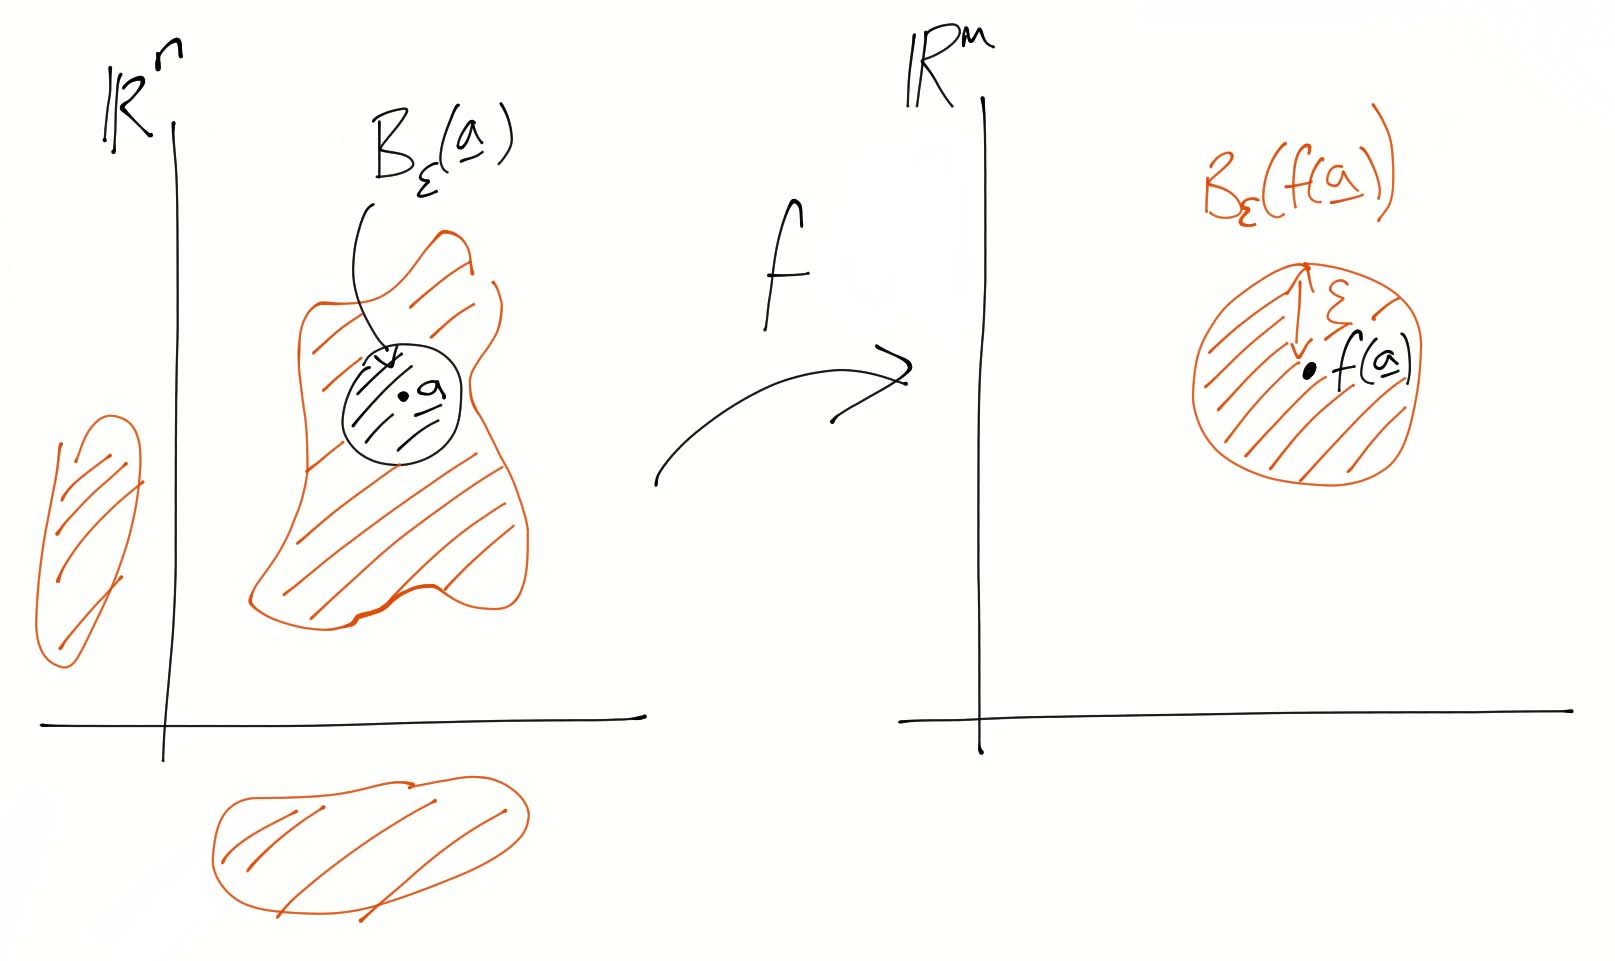
\includegraphics[width = 12cm]{ball1.jpg}
\end{center}


$f^{-1}(B_\epsilon(f(\vec{a}))) := \{\vec{x} \in \RR^n : f(\vec{x}) \in B_\epsilon (f(\vec{a}))\}$

Continuity at $\vec{a}$ says that $\vec{a}$ is in the ``interior'' of $f^{-1}(B_\epsilon (f(\vec{a})))$, i.e. $\exists$ a small ball $B_\delta (\vec{a})$ around it which is also in $f^{-1}(B_\epsilon(f(\vec{a})))$. 

So continuity at $\vec{a} \iff$ If $\vec{x}$ moves a tiny bit around $\vec{a}$ then $f(\vec{x})$ moves a tiny bit around $f(\vec{a})$.\pagebreak

\begin{example}
$f(x) = \begin{cases}
 	x\sin 1/x & x \neq 0\\
 	0 & x = 0
 \end{cases}$

\begin{center}
\begin{tikzpicture}
\begin{axis}[
axis lines=middle,
xtick = 0,
ytick = 0,
  width=10cm,height=5cm]
   \addplot[color = red, domain=-0.003:0.003,samples=500]{x*sin(1/x)};
   \addplot[domain=-0.003:0.003,smooth]{x};
   \addplot[domain=-0.003:0.003,smooth]{-x};
   \draw node at (axis cs: 0.0025,0.0028) {$x$};
   \draw node at (axis cs: 0.0025,-0.0028) {$-x$};
 \end{axis}
\end{tikzpicture}
\end{center}


\begin{proposition}
$f$ is continuous at $0$	
\end{proposition}

\begin{proof}
Fix $\epsilon >0$. Then 
\[|f(x) - f(0) = |x\sin\frac{1}{x}| \leq |x|\]
Take $\delta = \epsilon$. Then $|x| < \delta \implies |x| < \epsilon \implies |f(x) - f(0)| < \epsilon$	
\end{proof}
\end{example}\vspace*{5pt}

\begin{proposition}
$E: \CC \to \CC$ defined by $E(z) := \sum_{n=0}^{\infty} \frac{z^n}{n!}$ is continuous (i.e. continuous at $a,~\forall a \iC$)	
\end{proposition}
[Ex: from this show that $x \mapsto \sin x$ is continuous on $\RR$]

\emph{Rough working:} 
\[\begin{aligned}
|E(z) - E(a)| &= |E(a)(E(z-a)-E(0))| \\ 	
&= |E(a)| |E(z-a) -1|\\
& \leq |E(a)| \cdot \frac{|z-a|}{1-|z-a|}
\end{aligned}
\]
for $|z-a| < 1$ (see earlier lecture)
\[\begin{aligned}
\text{We want this to be } < \epsilon &\iff |z-a| < \frac{\epsilon}{|E(a)|}(1-|z-a|)\\
&\iff (1 + \epsilon/|E(a)|)|z-a| < \frac{\epsilon}{|E(a)|}\\
&\iff |z-a| < \epsilon/|E(a)|/(1 + \epsilon/|E(a)|)
\end{aligned}
\]


\begin{proof}
Fix $\epsilon >0$. Set $\delta = \dfrac{\epsilon}{|E(a)| + \epsilon} ~(*)$

Then we calculate that 
\[\begin{aligned}
|E(z) - E(a)| &\leq |E(a)| \frac{|z-a|}{1-|z-a|} \\
&< |E(a)| \cdot \frac{\delta}{1-\delta}	
\end{aligned}
\]	
for all $z$ with $|z-a| < \delta$. But by $(*)$, $\dfrac{\delta}{1-\delta} = \dfrac{\epsilon}{|E(a)|}$. 

So $|z-a|< \delta \implies |E(z) - E(a)| < \epsilon$.
\end{proof}~


\begin{theorem}
$f,g: \RR \to \RR$ cts at $a \in \RR \implies (f + g), f\cdot g$ are cts at $a$.
\end{theorem}
\begin{proof}
	Fix $\epsilon >0.$ \[\exists \delta_1 >0 \text{ such that }|x-a| < \delta_1 \implies |f(x) - f(a)| < \epsilon\] and\[\exists \delta_2 >0 \text{ such that }|x-a| < \delta_1 \implies |g(x) - g(a)| < \epsilon\]
	 Set $\delta =$ min$\{\delta_1,\delta_2\}.$ Then $\forall x$ such that $|x-a| < \delta:$
	\[|(f+g)(x) - (f+g)(a)| \leq |f(x) - f(a)| + |g(x) - g(a)| < 2\epsilon\]
	
	For (2): Similarly
	\[|f(x)g(x) - f(a)g(a)| \leq |g(x)||f(x) - f(a)| + |f(a)||g(x) - g(a)| ~(*)\]
	
	We need a bound on $|g(x)|$. We cannot bound $g(x)~ \forall x$!  But near $a$, $g(x)$ is close to $g(a)$, so we can bound $g(x)$ near $a$
	
	Take $\epsilon =1$ 
	\[\exists \delta_1 > 0\text{ s.t. }|x-a| < \delta_1 \implies |g(x) - g(a)| < 1 \implies |g(x)| < 1 + |g(a)| ~(A)\]
	
	Now fix any $\epsilon >0$. Then 
	\[\exists \delta_2 > 0\text{ s.t. }|x-a| < \delta_2 \implies |f(x) - f(a)| < \epsilon/1+|g(a)| ~ (B)\] (to cancel $|g(x)| < 1+|g(a)|$ in $(*)$)
	
	\[\exists \delta_3 > 0 \text{ s.t. } |x-a| < \delta_3 \implies |g(x) - g(a)| < \frac{\epsilon}{1 + |f(a)|}~ (C)\]
	(to cancel $|f(a)|$ in $(*)$)
	
	Set $\delta := \mathrm{min}\{\delta_1,\delta_2,\delta_3\}$. Then $|x-a| < \delta \implies (A), (B), (C)$ all hold. 
	
	Substitute into $(*)$ to find 
	\[\begin{aligned}|f(x)g(x) - f(a)g(a)| &< 1+|g(a)|\frac{\epsilon}{1+|g(a)|} + |f(a)|\frac{\epsilon}{1 + |f(a)|}\\
	&\leq \epsilon + \epsilon = 2\epsilon
\end{aligned}\]
\end{proof}


\begin{theorem}
	$f:\RR \to \RR$ cts at $a \in \RR$, $g:\RR \to \RR$ cts at $f(a) \in \RR$, then $g \circ f$ cts at $a$
\end{theorem}

\emph{Idea of Proof:} We want $g(f(x))$ to be close (within $\epsilon$) to $g(f(a))$. 

But $g$ is continuous at $f(a)$! So sufficient for $f(x)$ to be close (within $\delta_g$ to $f(a)$. But $f$ is continuous at $a$! so we can arrange this (by taking $\epsilon = \delta_g$ by taking $x$ to be close (within $\delta_g$) to $a$. 

\begin{proof}\lecturemarker{20}{5 Oct}
Fix $\epsilon >0.$ $g$ is continuous at $f(a)$, so \[\exists \delta > 0\text{ s.t. }|g - f(a)| < \delta \implies |g(y) - g(f(a))| < \epsilon\]

Also $f$ is continuous at $a$, so 
\[\exists \eta > 0\text{ s.t. }|x-a| < \eta \implies |f(x) - f(a)| < \delta\]

\noindent Hence $|x-a| < \eta \implies |f(x) - f(a)| < \delta \implies |g(f(x)) - g(f(a))| < \epsilon.$
\end{proof}

\begin{corollary}
$a^x:= E(x\log a), ~a>0$ is continuous $\forall x \iR$	
\end{corollary}
\begin{proof}
It is a composition $\displaystyle{\RR \xrightarrow[x \mapsto x\log a]{} \RR \xrightarrow[y \mapsto E(y)]{} \RR }$ of two functions.	
\end{proof}

Ex: Show $\sin 1/x$ is continuous for $\RR\backslash\{0\} \to \RR$. (i.e. show $1/x$ is continuous from first principles, $\sin x$ is continuous using continuity of $E(x)$ and compose!)\vspace*{15pt}

\begin{example}
Suppose $f:\RR\to \RR\backslash\{0\}$ is continuous. Then $1/f$ is continuous. 

\begin{proof}
Pick $a\iR$. Show $1/f(x)$ is continuous at $a$: 

\[\left|\frac{1}{f(x)} - \frac{1}{f(a)}\right|  = \frac{1}{|f(x)f(a)|}|f(x)-f(a)| ~(*)\]

We need to bound $f(x)$ below! Need $|f(x)| > \text{ some }\eta > 0 \iff \frac{1}{|f(x)|} < \frac{1}{\eta}$

We can't, but we can near $a$! $f(a) \neq 0$, so take $\epsilon' = |f(a)|/2 >0$. Then 
\[\exists \delta' \text{ s.t. } |x-a| < \delta' \implies|f(x) - f(a)| < \epsilon' = \frac{|f(a)|}{2}\]
\[\implies |f(x)| > |f(a)| -\epsilon = \frac{|f(a)|}{2}\]


\[\begin{aligned}
\text{So by } (*) \text{, we have }\left|\frac{1}{f(x)} - \frac{1}{f(a)}\right| &< \frac{1}{|f(a)|/2\cdot |f(a)|} |f(x) - f(a)| \\ 
	& = \frac{2}{|f(a)|^2}|f(x) - f(a)|
\end{aligned}
\]

Fix $\epsilon >0$. Set $\epsilon'' = \mathrm{min}\left(\frac{|f(a)|}{2}, \frac{\epsilon}{2}|f(a)|^2\right) > 0$

Then $\exists \delta > 0$ such that $|x-a| < \delta \implies |f(x) - f(a)| < \epsilon''$ (by continuity of $f$ at $a$)

$\implies (1) |f(x)| > |f(a)| - \epsilon'' \geq |f(a)| - |f(a)|/2$ and $(2) |f(x) - f(a)| < \frac{\epsilon}{2}|f(a)|^2$. So 

\[\begin{aligned}
\left|\frac{1}{f(x)} - \frac{1}{f(a)}\right| &= \frac{1}{|f(x)||f(a)|} |f(x) -f(a)| \\
&< \frac{1}{|f(a)|/2\cdot|f(a)|}\cdot \frac{\epsilon}{2}|f(a)|^2 = \epsilon	\qedhere
\end{aligned}
\]
\end{proof}	
\end{example}


\begin{theorem}
	$f: \RR \to \RR$ is cts at $a \in \RR$ iff $\forall$ sequences $x_n \to a$, $f(x_n) \to f(a)$
\end{theorem}

In one direction this is somewhat easy: if $x_n \to a$ and $f$ is continuous at $a$, then $f(x_n)$ gets close to $f(a0$ as $x_n$ gets close to $a \implies f(x_n) \to f(a)$. 

The converse is \emph{much harder}. If I want to see if $f$ is continuous, I can test with a sequence $x_n \to a$ to see if $f(x_n)$ if close to $f(a)$ when $n$ is large. But $x_n$'s doesn't cover all $x$'s! But if I use \emph{all} sequences $x_n \to a$ then I do cover all $x$ and get a theorem. 

\begin{proof}
If $f$ is cts at $a$, fix $\epsilon >0$. $\exists \delta > 0$ such that $|x-a| < \delta \implies |f(x) - f(a)| < \epsilon$. Now $x_n \to a$, so $\exists N \in \mathbb{N}$ such that $n \geq N \implies |x_n - a| < \delta \implies |f(x_n) - f(a)| < \epsilon$.\\

\noindent Suppose $f$ is not cts at $a\in \RR$ for contradiction.

 Then $\exists \epsilon >0$ such that $\forall \delta >0,~\exists x \in (a-\delta,a+\delta)$ such that $|f(x) -f(a)| \geq \epsilon.$ 
 
 Choose $\delta = \frac{1}{n}$. $\exists x_n \in (a - \frac{1}{n},a + \frac{1}{n})$ such that $|f(x_n) - f(a)| \geq \epsilon$. 
 
 So $|x_n-a| < \frac{1}{n}~\forall n \implies x_n \to a$. But $f(x_n) \centernot\implies f(a),~\cont$.  
\end{proof}~

\begin{example}
$f(x) =\begin{cases}
\sin 1/x & x \neq 0\\
0 = 0
\end{cases}
$	

This is \emph{not} continuous at $0$. But if we take $x_n \to 0$, then $f(x_n) = \sin(n\pi) = 0~\forall n$, so $f(x_n)\to f(0)$. so this sequence does not defect. 

Have to choose a different sequence e.g. $x_n = \frac{2}{\pi},\frac{2}{3\pi},\frac{2}{5\pi},\dots,$ gives $\sin\frac{1}{x_n} = (-1)^{n+1} \not\to f(0) \implies f$ discontinuous at $0$.  
\end{example}

To get this problem of sequences not covering the whole of an interval $(a-\delta, a+\delta)$ (so having to consider all sequences at once - nasty), we can let $x$ run through all of $\RR$ with the following definition:\\

\begin{definition}\lecturemarker{21}{5 Oct}
$f: \RR\to \RR$, $a\iR$. 

We say that $f(x) \to b$ as $x \to a$ (or ``$\lim_{x\to a} f(x) = b$'') iff 
\[\forall \epsilon >0,~\exists \delta > 0 \text{ s.t. } 0 < |x-a| < \delta \implies |f(x) - b| < \epsilon\]	
\end{definition}

``$x$ close to $a$ (but not equal!!) $\implies f(x)$ close to $b$''\vspace*{15pt}

\begin{example}
$f(x) = \begin{cases}
 0 & x \neq 0\\
 1 & x=0	
 \end{cases}$
	
Then $\lim_{x\to 0} f(x) = 0$

e.g. We can talk about $\lim_{x\to 0}f(x)$ for $f: \RR\backslash\{0\} \to \RR$.
\end{example}

\begin{theorem}
$f: \RR \to \RR$ is continuous at $a \iR$ iff $f(x) \to f(a)$ as $x \to a$	
\end{theorem}

\begin{proof}
$f$ is continuous at $a\iR$ says (1):
\[\forall \epsilon > 0,~\exists \delta > 0 \text{ s.t. } |x-a| < \delta \implies |f(x) - f(a)| < \epsilon\]

Whereas $f(x) \to f(a)$ as $x \to a$ says (2):
\[\forall \epsilon > 0,~\exists \delta > 0 \text{ s.t. } 0 < |x-a| < \delta \implies |f(x) - f(a)| < \epsilon\]

So (1)$\implies$ (2).

Suppose (2). Then I get (1) except for when $|x-a| = 0$. But when $|x-a| = 0$, then $x=a$, so $f(x) = f(a)$, so $|f(x) - f(a)| < \epsilon$, so I still get (1).
\end{proof}


Can extend the definition of continuity to functions defined on subsets of $\RR$ or $\RR^n$ e.g.\vspace*{10pt}
\begin{definition}
$f: S \to \RR^m$, $S \subseteq \RR^n$, is continuous at $\vec{a} \in S$ iff
\[\forall \epsilon > 0,~\exists \delta > 0 \text{ s.t. } (0 < |\vec{x}-\vec{a}| < \delta \text{ and } x \in S) \implies |f(\vec{x}) - f(\vec{a})| < \epsilon\]
\end{definition}\vspace*{5pt}

\begin{example} 
$f: \RR \to \RR$, $f(x) = \begin{cases}
 0 & x \iQ\\
 1 & x \not\in\QQ	
 \end{cases}$
 
 This is discontinuous. But $\left.f\right|_\QQ: \QQ \to \RR$ is continuous. 	
\end{example}

Related to this is one-sided continuity:\\

\begin{definition}
$f: \RR \to \RR$ is \emph{right continuous} at $a\iR$ iff
\[\forall \epsilon > 0,~\exists \delta > 0 \text{ s.t. } x \in [a, a+\delta) \implies |f(x) - f(a)| < \epsilon\]
\end{definition}

Ex: $f$ is right continuous at $a \in \RR \iff \left. f \right|_{[a,\infty)}: [a,\infty) \to \RR$ is continuous at $a \in \RR$. 

Ex: $f: \RR \to \RR$ is continuous at $a\iR \iff f$ is both right and left continuous at $a \iR$\\

\begin{definition}
	$f(x) \to b$ as $x \to a_+$ ``as $x$ tends to $a$ from above''
	means 
	\[\forall \epsilon > 0,~\exists \delta > 0 \text{ s.t. } x \in (a,a+\delta) \implies |f(x) - f(a)| < \epsilon\]
\end{definition}

Ex: Just as before find that $f$ is right continuous at $a\iff f(x) \to f(a)$ as $x \to a_+$

\pagebreak
\subsektion{Intermediate Value Theorem}\vspace*{5pt}

\begin{theorem}[Intermediate Value Theorem] If $f: [a,b] \to \RR$ cts, $c \in (f(a),f(b)),$ then $\exists x \in [a,b]$ such that $f(x) = c$
\end{theorem}

\begin{center}
\begin{tikzpicture}
\begin{axis}[
 axis line style={red},
 axis lines=middle,
   %  x label style={at={(axis description cs:1.05,0.4)}},
   %  y label style={at={(axis description cs:-0.08,1.02)}},
  ymin = -0.2,
  ymax = 1,
  xmin = 1,
  xmax = 10,
     ytick = {0.5},
   yticklabels={$c$},
   xtick = 0,
  width=12cm,height=6.5cm]
   \addplot[draw=blue, domain=4:5,smooth] {(0.0309*x^3 - 0.5504*x^2 + 3.313*x - 6.23)};
      \addplot[draw=blue, domain=7:8,smooth] {(0.0309*x^3 - 0.5504*x^2 + 3.313*x - 6.23)};
       \draw[dashed] (axis cs:20,0.5) -- (axis cs:0,0.5); %c line
                        \draw (axis cs:6,0.04) -- (axis cs:6,-0.04)  node at (axis cs:6,-0.1) {$x$};
                     \draw (axis cs:4,0.04) -- (axis cs:4,-0.04)  node at (axis cs:4,-0.1) {$a$};
                        \draw (axis cs:8,0.04) -- (axis cs:8,-0.04)  node at (axis cs:8,-0.1) {$b$};

  \end{axis}
\end{tikzpicture}
\end{center}


If $f$ is continuous it must cross the line $y=c$ at some point $x \in [a,b]$. 

\begin{corollary}
Any odd degree polynomial over $\RR$ has a root $\iR$	
\end{corollary}
\begin{proof}
w.l.o.g. $p(x) = x^{2n+1} + a_{2n}x^{2n} + \dots + a_1x + a_0$

If we write this as $p(x) = x^{2n+1}(1 + \frac{a_{2n}}{x} + \dots + \frac{a_0}{x^{2n+1}})$ then we see that $p(x) < 0$ for $x << 0$, and $p(x) > 0$ for $x>>0$. 

So we can find $a,b \iR$ such that $p(a) < 0$,  $p(b) > 0$. 

So we apply IVT to $\left.p\right|_{[a,b]}: [a,b] \to \RR$ with $c = 0$ to find an $x \in [a,b]$ with $p(x) = c = 0$.
\end{proof}

We used the facts (proved in earlier lectures) that $mx +c$ is continuous and the product/sum of continuous functions are also continuous $\implies p(x)$ is continuous. 

\begin{proof}[Proof of IVT]\lecturemarker{22}{5 Oct}

\begin{center}
\begin{tikzpicture}
\begin{axis}[
 axis line style={red},
 axis lines=middle,
  ymin = -0.2,
  ymax = 1,
  xmin = 1,
  xmax = 10,
     ytick = {0.6, 0.25, 0.95},
   yticklabels={$c$, $f(a)$, $f(b)$},
   xtick = 0,
  width=12cm,height=7cm]
      \addplot[draw=blue, domain=4:9,smooth]{0.006*x^4 - 0.0987*x^3 + 0.3937*x^2 + 0.6556*x - 3.9};
            \addplot[thick, domain=6.5:8.054,smooth]{0.006*x^4 - 0.0987*x^3 + 0.3937*x^2 + 0.6556*x - 3.9};
               \addplot[thick, domain=4:4.849,smooth]{0.006*x^4 - 0.0987*x^3 + 0.3937*x^2 + 0.6556*x - 3.9};
       \draw (axis cs:20,0.6) -- (axis cs:0,0.6); %c line
       \draw[dotted] (axis cs:4.849,0.04) -- (axis cs:4.849,-0.04)  node at (axis cs:4.5,-0.1) {$S_c$};
       \draw[dotted] (axis cs:4,0.25) -- (axis cs:4,-0.04)  node at (axis cs:4,-0.1) {$a$};
       \draw[dotted] (axis cs:8.054,0.6) -- (axis cs:8.054,-0.04) node at (axis cs: 8.8,-0.1) {$b$};
       \draw[dotted] (axis cs:6.5,0.6) -- (axis cs:6.5,-0.04)  node at (axis cs:7.3,-0.1) {$S_c$};
        \draw (axis cs:8.8,0.04) -- (axis cs:8.8,-0.04);
        \draw (axis cs:4,0.04) -- (axis cs:4,-0.04);
  \end{axis}
\end{tikzpicture}
\end{center}

Consider $S_c = \{y \in [a,b] : f(y) \leq c\}$. Define $x:=$ sup$S_c$ ($S_c \neq \emptyset$ since $a \in S_c$ and bounded above by $b$ so sup exists)

\textbf{Claim: $f(x) = c$}. \textit{Proof:} \begin{enumerate}
 \item Suppose $f(x) < c$. 
 
\begin{center}
\begin{tikzpicture}
\begin{axis}[
 axis line style={red},
 axis lines=middle,
   %  x label style={at={(axis description cs:1.05,0.4)}},
   %  y label style={at={(axis description cs:-0.08,1.02)}},
  ymin = -0.2,
  ymax = 1,
  xmin = 1,
  xmax = 10,
     ytick = {0.6,0.4},
   yticklabels={$c$,$f(x)$},
   xtick = 0,
  width=12cm,height=7cm]
   \addplot[draw=blue, domain=4:8,smooth] {(0.0309*x^3 - 0.5504*x^2 + 3.313*x - 6.23)};
   %\addplot {(6,0.55)};
   \addplot [color=black, mark=*, mark options={solid},]
                coordinates{(6,0.5)};
       \draw(axis cs:20,0.6) -- (axis cs:0,0.6); %c line
        \draw[dotted] (axis cs:20,0.4) -- (axis cs:0,0.4); %fx line
        \draw (axis cs:6,0.04) -- (axis cs:6,-0.04)  node at (axis cs:6,-0.1) {$y \in S_c,\cont$};
       \draw (axis cs:4.7,0.04) -- (axis cs:4.7,-0.04)  node at (axis cs:4.7,-0.1) {$x$};
     \draw[<->] (axis cs:7,0.5) -- (axis cs:7,0.6) node at (axis cs:8.2,0.55) {$\epsilon = c-f(x)$};
     \draw node at (axis cs: 6.2, 0.42) {$f(y)$};
  \end{axis}
\end{tikzpicture}
\end{center}
 
 
 Take $\epsilon = c-f(x) > 0$. $f$ is cts at $x$, so $\exists \delta > 0$ such that $\forall y \in (x,x+\delta) \cap [a,b], ~|f(y) - f(x)| < \epsilon$. Hence $f(y) < f(x) + \epsilon = c$. So $y\in S_c \implies x \neq$ sup$S_c$.\\
 
 \item 	Suppose $f(x) > c$.
 
\begin{center}
\begin{tikzpicture}
\begin{axis}[
 axis line style={red},
 axis lines=middle,
   %  x label style={at={(axis description cs:1.05,0.4)}},
   %  y label style={at={(axis description cs:-0.08,1.02)}},
  ymin = -0.2,
  ymax = 1,
  xmin = 1,
  xmax = 10,
     ytick = {0.55},
   yticklabels={$c$},
   xtick = 0,
  width=12cm,height=7cm]
   \addplot[draw=blue, domain=4:8,smooth] {(0.0309*x^3 - 0.5504*x^2 + 3.313*x - 6)};
      \addplot [color=black, mark=*, mark options={solid},]
                coordinates{(6,0.73)};
       \draw (axis cs:20,0.55) -- (axis cs:0,0.55); %c line
                        \draw (axis cs:6,0.04) -- (axis cs:6,-0.04)  node at (axis cs:6,-0.1) {$x$};
                     \draw (axis cs:4.4,0.04) -- (axis cs:4.4,-0.04)  node at (axis cs:4.5,-0.1) {$a$};
                \draw[<->] (axis cs:7,0.73) -- (axis cs:7,0.55) node at (axis cs:8.2,0.6) {$\epsilon = f(x)-c$};
                \draw node at (axis cs: 6.2, 0.66) {$f(x)$};
  \end{axis}
\end{tikzpicture}
\end{center}

  
  Take $\epsilon = f(x)-c > 0$. $f$ is cts at $x$, so $\exists \delta > 0$ such that $\forall y \in (x-\delta,x) \cap [a,b], ~|f(y) - f(x)| < \epsilon$. Hence $f(y) > f(x) - \epsilon = c \implies x- \delta$ is an upperbound for $S_c$, so $x \neq$ sup$S_c$. \qedhere
 \end{enumerate}
\end{proof}\vspace*{5pt}

\begin{proposition}
Suppose $f: [0,1] \to [0,1]$ is continuous. Then it has a fixed point (i.e. $\exists x \in [0,1]$ s.t. $f(x) = x$)	
\end{proposition}

\emph{Idea of proof:} Rotate picture to make it look like IVT. 

\begin{center}
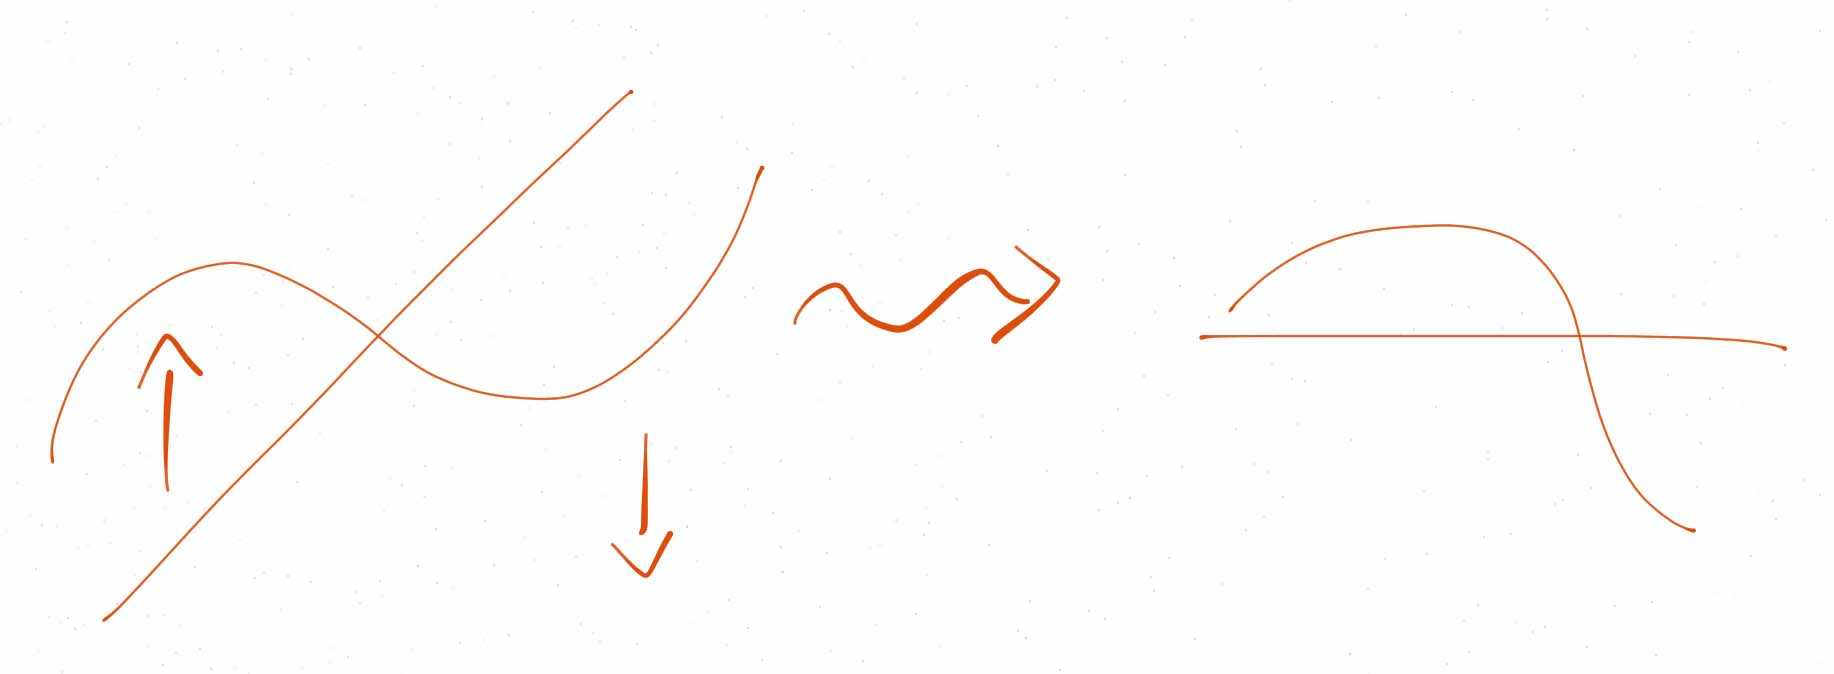
\includegraphics[width = 12cm]{rotate.jpg}
\end{center}

\begin{proof}
Set $g(x) = f(x) - x$, $g: [0,1] \to [0,1]$ is continuous. 

So $g(0) = f(0) - 0 \geq 0$, $g(1) = f(1) -1 \leq 0$

So by IVT $\exists x\in[0,1]$ s.t. $g(x) = 0\iff f(x) = x$	
\end{proof}

So if during the lecture you watch last weeks lecture on Panopto, using pause, fast-forward, rewind, play (but no jumping!) then at some point you will be watching a time in the lecture which equals the time now. (No matter where you start or end.) \\

\begin{definition}
	$S \subseteq \RR^n$,$f: S \to\RR$. Then we say that $f$ is bounded above if $\exists M \iR$ s.t. $f(\vec{x}) \leq M$ $\forall \vec{x} \in S$. 
	
	Similar for bounded below, bounded is both. 
\end{definition}

\begin{example}
$f(x) = \frac{1}{x}: (0,1] \to \RR$ is not bounded above

\begin{proof}
Suppose $\frac{1}{x} \leq M~\forall x\in(0,1]$ (Then $M > 0!$).
 
Then take $x = \mathrm{min}\{\frac{1}{2m},1) \implies x \leq 1/2m \implies 1/x \geq 2M > M,~\cont$.
\end{proof}	
\end{example}

Also $f(x) = \begin{cases}
 \frac{1}{x} & x\neq 0\\
 0 & x = 0	
 \end{cases}$
 
 $f:[0,1]\to \RR$ is also unbounded. Note that $f$ is not continuous at 0!
 
 So $\begin{cases}
	\mbox{discontinuous functions can be unbounded}\\
	\mbox{continuous functions can be unbounded on non-closed intervals}
\end{cases}$

But..

\begin{theorem}
$f:[a,b] \to \RR$ cts $\implies f$ is bounded.	
\end{theorem}

Ex: Give a function $f: [a,b] \cap \QQ \to \RR$ which is continuous and unbounded. 

\begin{proof}[Proof]\lecturemarker{23}{5 Oct}
Suppose not. Then $\forall N \in \mathbb{N}$, $N$ is not an unpperbound, so $\exists x_N \in [a,b]$ such that $|f(x_n)| > N$.

By BW Theorem, exists convergent subsequence, $y_i := x_{N(i)}, y_i \to y \in [a,b]$. With $|f(y_i)| = |f(x_{N(i)})| > N(i) \geq i ~(*)$. 

Fix $\epsilon =1$, then 
\[\exists \delta > 0\text{ such that }\forall x \in (y-\delta, y + \delta): |f(x) - f(y)| < 1 \implies |f(x)| < |f(y)| +1.\]
 Since $y_i \to y$, 
 \[\exists N\text{ such that }\forall n \geq N~ |y_n - y| < \delta \implies y_n \in (y-\delta, y + \delta) \implies |f(y_n)| < |f(y)| + 1.\]
 
 By $(*)$, $n \leq |f(y_n)| < |f(y)| + 1~ \forall n \geq N$, not true by the Archimedean Axiom $\cont$.
\end{proof}

\begin{proof}[Slicker Proof]
	Suppose not. Then $\forall N \in \mathbb{N}$, $N$ is not an unpperbound, so $\exists x_N \in [a,b]$ such that $|f(x_n)| > N$.
	
By BW Theorem, exists cvgt subsequence, $y_i := x_{N(i)}, y_i \to y \in [a,b]$. With $|f(y_i)| = |f(x_{N(i)})| > N(i) \geq i ~(*)$. $f$ is cts at $y \implies f(y_i) \to f(y)$, contradicting $(*)$.  
\end{proof}\vspace*{5pt}


\subsektion{Extreme Value Theorem}\vspace*{5pt}
\begin{theorem}[Extreme Value Theorem] $f: [a,b] \to \RR$ cts $\implies f$ bounded and attains its bounds.
\end{theorem}

So max $f(x)$ exists (not just sup)

\begin{proof}[Proof]
	By boundedness theorem, $\exists \displaystyle{\text{sup}_{x \in [a,b]}} f(x) = s$. Suppose for contradiction $\not \exists c \in [a,b]$ such that $f(x) = s$. 
	
	\emph{2 proofs}:
	
	(1) Then $s-f(x) > 0 ~\forall x \in [a,b],$ so $g(x) = \frac{1}{s-f(x)}: [a,b] \to \RR$ is well defined and cts. So $g(x)$ is bounded by $M > 0 \implies \frac{1}{s-f(x)} \leq M \implies f(x) \leq s - \frac{1}{M}$, so $s \neq$ sup$f(x),~\cont$.\vspace*{10pt}

	(2) From M1F $\exists$ a sequence $x_n \in [a,b]$ such that $f(x) \to  \displaystyle{\text{sup}_{x \in [a,b]}} f(x) = s$. BW Theorem $\implies$ exists subsequence $y_i := x_{N(i)}$ such that $y_i \to c \in [a,b].$ $f$ is cts $\implies f(y_i) \to f(x)$. Since $f(y_i) \to s$, by uniqueness of limits, $f(c) = s$.
	\end{proof}
	
	Combining IVT + EVT we get
	
	\begin{theorem}
	$f: [a,b] \to \RR$ is continuous then $\exists c,d \in [a,b]$ s.t. im$f = f[a,b]$ is the interval $[f(c),f(d)]$. 	
	\end{theorem}
	
	\begin{proof}
	EVT $\implies \exists c,d$ s.t. $f[a,b] \subseteq [f(c),f(d)] ~(*)$
	
	Given any $y \in [f(c),f(d)]$ the IVT $\implies \exists x$ between $c$ and $d$ s.t. $f(x) = y$, so $(*)$ is onto.	
	\end{proof}

\subsektion{Inverse Function Theorem}\vspace*{5pt}

\begin{proposition}
If $f:[a,b]\to\RR$ is continuous and strictly increasing ($x>y \implies f(x) > f(y)$), then $f$ is a bijection $[a,b] \to [f(a),f(b)]$	
\end{proposition}
\begin{proof}
$f(a)$ is a minimum of $f[a,b]$ because $x>a\implies f(x) > f(a)$. $f(b)$ is maximum. So by previous result $f[a,b] = [f(a), f(b)]$. We just need too show that $f$ is injective: 

If $x \neq y$, w.l.o.g. $x \neq y$ then $x < y \implies f(x) < f(y) \implies f(x) \neq f(y)$. So $f$ is injective. 
\end{proof}

So $\exists$ inverse $g := f^{-1}: [f(a),f(b)] \to [a,b]$

\begin{proposition}
$g$ is continuous (and also strictly increasing - Ex!)	
\end{proposition}

\begin{proof}
Fix $\epsilon >0$ and $y_0 \in [f(a),f(b)]$. 

Set $\delta:= \mathrm{min}(f(g(y_0) + \epsilon) - f(g(y_0)), f(g(y_0)) - f(g(y_0) - \epsilon))$

$ = \mathrm{min}(f(x_0 + \epsilon) -  y_0, y_0 - f(x-\epsilon))$	 where $x_0 = g(y_0)$

\emph{Picture:} 
\begin{center}
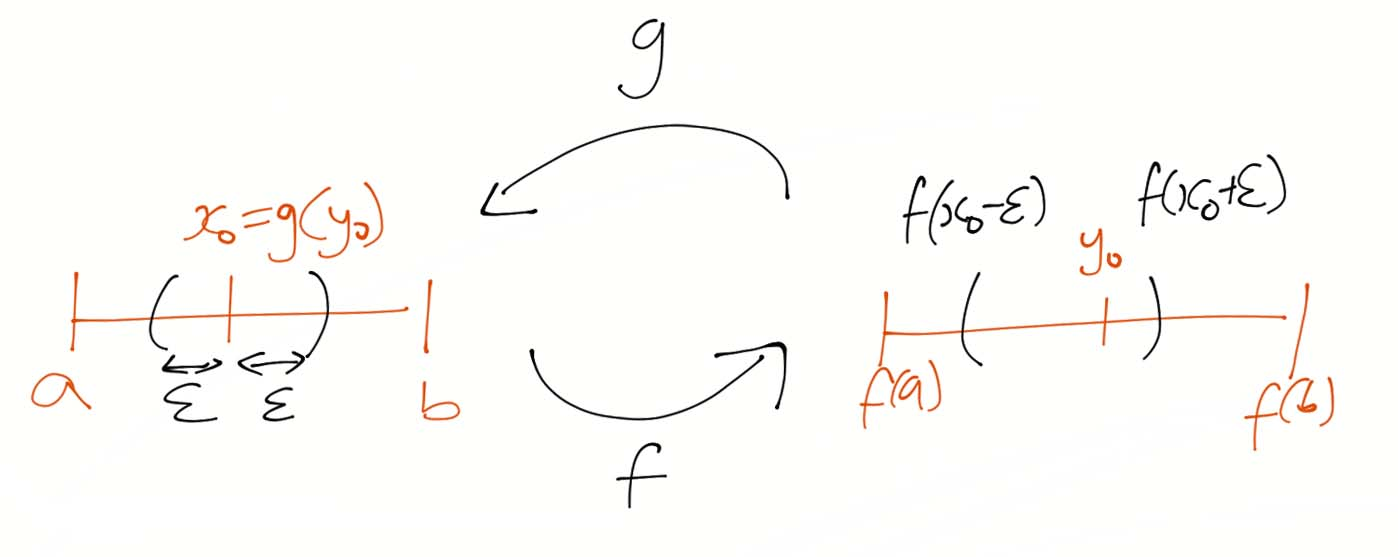
\includegraphics[width = 12cm]{ball2.jpg}
\end{center}

In this definition we use the convention that if $x_0 -\epsilon <a$ then by $f(x_) - \epsilon$ I mean $f(a)$ if $x_0 + \epsilon > b$ then $f(x_0 + \epsilon)$ means $f(b)$. 

(Equivalently I've extended $f$ to $\tilde f: \RR \to \RR$ by $\tilde f(x) =\begin{cases}
f(a) & x \leq a\\
f(x) & x \in [a,b]\\
f(b) & x \geq b
\end{cases}
$)

So $\delta$ was chosen s.t. $(y_0 -\delta, y_0 + \delta) \subseteq (f(x_0 - \epsilon), f(x+\epsilon))$, so $y \in (y_0 - \delta, y_0 + \delta) \cap [a,b]$ then $f(x_0 -\epsilon) < y < f(x_0 + \epsilon)$

Apply $g\implies x_0 -\epsilon < g(y) < x_0 + \epsilon$. Recall $x_0 = g(y_0) \implies |g(y) - g(y_0)| < \epsilon$.
\end{proof}

\begin{corollary}
$\sqrt{x}: [0,\infty) \to [0,\infty)$, $x^{1/n}: [0,\infty) \to [0,\infty),~n\iN$ are continuous. 	
\end{corollary}

Simpler exposition: Fix $f: \RR \to \RR$ bijective and continuous. Before we prove $f^{-1}$ is continuous we prove

\begin{lemma}\lecturemarker{24}{5 Oct}
$f:\RR \to \RR$ is bijective and cts $\implies f$ is strictly monotonic	
\end{lemma}

\begin{proof}
We prove this on any closed bounded interval $[a,b]$ (Hence monotonic on $\RR!$ Ex!)

$f$ is bijective, so $f(a) \neq f(b)$, w.l.o.g. $f(b) > f(a).$ Suppose for contradiction $\exists c \in (a,b)$ such that $f(c) \not\in (f(a),f(b)).$ 

w.l.o.g. take $f(c) > f(b)$. Then fix $d \in (f(b),f(c))$. By IVT applied to:
\begin{itemize} 
\item $f|_{[a,c]}$, we find $\exists x \in (a,c)$ such that $f(x) = d$. 
\item $f|_{[c,b]}$, we find $\exists y \in (c,b)$ such that $f(y) = d$.
	
\end{itemize}
But $y > x \implies x  \neq y$, so $f$ is not injective $\cont$. 

So $\forall c \leq b$, we find that $f(c) \leq f(b)$, and $f$ injective $\implies f(c) < f(b)$. 
\end{proof}\vspace*{5pt}

\begin{theorem}
	$f: \RR \to \RR$ bijective and cts $\implies f^{-1}: \RR \to \RR$ cts.
\end{theorem}
\begin{proof}
By Lemma $f$ is strictly monotonic, w.l.o.g. strictly increasing. 

We want to show $f^{-1}$ is continuous at $y\iR$. Let $x_0 \iR$ be $f^{-1}(y_0)$, so $f(x_0) = y_0$.

Fix $\epsilon > 0$.

Let $\delta :=$ min$\{f(x_0 + \epsilon) - y_0, y_0 - f(x_0 - \epsilon)\}$. 
 
 Then $|y -  y_0| < \delta \implies y \in (y_0 -\delta, y_0 + \delta) \subseteq (f(x_0 - \epsilon), f(x_0 + \epsilon))$. 
 
 Applying $f^{-1}$ preserves order \[\implies f^{-1}(y) \in (x_0 - \epsilon, x_0 + \epsilon) \iff |f^{-1}(y) - f^{-1}(y_0)| < \epsilon.\qedhere\]
\end{proof}\vspace*{5pt}

\begin{corollary}
$E:\RR \to \RR$, $E(x): \sum \frac{x^n}{n!}$ is a continuous bijection $\RR \to (0,\infty)$ with continuous inverse $\log: (0,\infty) \to \RR$. 	
\end{corollary}\vspace*{5pt}

We already showed that $E$ is continuous, never takes the value $0$ ($E(-x) = E(x)^{-1}$) is unboundedly poisitive for $x \geq 0$ ($E(x) \geq 1 + x$) and positive for $x < 0$ ($E(-x) = E(x)^{-1}$). So by IVT it takes \emph{every} value in $(0,\infty)$ (Ex!). 

We also showed it is strictly monotonically increasing ($E(y) = E(y-x)E(x) > E(x)$ for $y > x$). So by previous result it's a bijection to $(0,\infty)$ with a continuous inverse.\vspace*{5pt}


\begin{theorem}\lecturemarker{25}{12 March}
	$f:\RR^n \to \RR^m$ is cts at $\mathbf{a} = (a_1,\dots,a_n)$ if and only if $f_i:\RR^n \to \RR$ is cts at $a_i~\forall i$. (With $f = (f_1,\dots,f_m)$).
\end{theorem}

(i.e. $f_i$ is $\pi_i \circ f$ where $\pi_i: \RR^m \to \RR$ is the projection to the $i$th coordinate $\pi_i(x_1,\dots,x_m) = x_i$.)

\begin{proof}

Easy way is $\implies$:

\textsc{Highbrow:} $\pi_i: \RR^m \to \RR$ is continuous, so $\pi_i \circ f - f_i$ is continuous.

\textsc{First Principles:}
	Fix $\epsilon >0.$ Then $f$ is cts at $\vec{a} \implies \exists \delta >0 $ such that $|\vec{x} - \vec{a}| < \delta  \implies |f(\vec{x}) - f(\vec{a})| < \epsilon ~(*)$. But this implies $|f_i(\vec{x}) - f_i(\vec{a})| < \epsilon$ because
	
\[\begin{aligned}
|f(\vec{x}) - f(\vec{a})| &= \sqrt{\sum_{j=1}^m (f_j(\vec{x}) - f_j(\vec{a}))^2}\\
&\geq \sqrt{(f_i(\vec{x}) - f_i(\vec{a}))^2}\\
&= |f_i(\vec{x}) - f_i(\vec{a})| 	
\end{aligned}
\]	
\textsc{Proof of $\impliedby$:}

	Suppose $f_i$ cts at $a_i~\forall i$. Fix $\epsilon > 0$. Then $\exists \delta_i > 0$ such that \[|\vec{x} - \vec{a}| < \delta_i \implies |f_i(\vec{x}) - f_i(\vec{a})| < \epsilon\]
	 Set $\delta =$ min$\{(\delta_i\} >0$, so that 
	 \[\begin{aligned}|\vec{x} - \vec{a}| < \delta &\implies |f_i(\vec{x}) - f_i(\vec{a})| < \epsilon ~\forall i\\
	  \implies |f(\vec{x}) - f(\vec{a})| &= \sqrt{\sum_{i=1}^m (f_i(\vec{x}) - f_i(\vec{a}))^2} \\
	  &\leq \sqrt{\sum_{i=1}^m \epsilon^2} = \sqrt{m}.\epsilon	
\end{aligned}
\]
\end{proof}

So we can study the continuity of $f: \RR^n \to \RR^m$ in terms of their coordinates $f_i$ in $\RR^m$. But \emph{not} in terms of the restoration of $f$ to coordinate axises in $\RR^n$.\vspace*{15pt}

\begin{example}
$f: \RR^2 \to \RR$, $f(x,y) = \begin{cases}
 	\dfrac{xy}{x^2 + y^2} & (x,y) \neq (0,0)\\
 	0 & (x,y) = (0,0)
 \end{cases}$
 
 On any horizontal line $y =c$ it results to the function 
 \[f(x,c) = \frac{cx}{c^2 + x^2} \quad \text{ if } c \neq 0\]
 \[\text{ or } f(x,0) \equiv 0 ~\forall x \quad \text{ if } c = 0\]
 Both are continuous functions $\RR \to \RR$. 
 
 Similarly on any vertical line $x = c$, $f$ restricts to a continuous function: 
  \[f(c,y) = \frac{cy}{c^2 + y^2} \quad \text{ if } c \neq 0\]
 \[\text{ or } f(0,y) \equiv 0 ~\forall y \quad \text{ if } c = 0\]
 But $f$ is \emph{not} continuous at $(0,0)$
 
 \emph{Idea:} on line $y=x$, $f$ is $\begin{cases}
	\dfrac{x.x}{x^2 + x^2} = \frac{1}{2} & \forall x \neq 0\\
	0 & x = 0
\end{cases}$

Pick $\epsilon = \frac{1}{2}$. Then for any $\delta > 0$, take $x = \frac{\delta}{2}$ so that $(x,x) \in B_\epsilon(0,0)$. But $f(x,x) = \frac{1}{2} \not\in B_\epsilon(f(0,0)) = B_\epsilon(0)$. So $f$ is not continuous at $(0,0)$. \qed
\end{example}

Ex: Converse is true: if $f: \RR^n \to \RR^m$ is continuous then $f$ is continuous on restriction to any line in $\RR^n$; more generally $\left.f\right|_S: S \to \RR^m \text{ is continuous } \forall S \subseteq \RR^n$



		% Continuity
%!TEX root = M1P1.tex

\stepcounter{lecture}
\setcounter{lecture}{4}

\pagebreak

\sektion{Differentiation}
\label{sub:differentiation}

\subsektion{Differentiability}\vspace*{5pt}

\begin{definition}
$f$ is \emph{differentiable}  at $a$ iff $\lim_{x\to a} \frac{f(x)-f(a)}{x-a} = f'(a)$, i.e.
\[\forall \epsilon > 0,~\exists \delta > 0\text{ such that } 0<|x-a| < \delta \implies \left|\frac{f(x)-f(a)}{x-a}-f'(a)\right| < \epsilon.\]	
\end{definition}

\begin{center}
\begin{tikzpicture}
\begin{axis}[
 axis line style={red},
 axis lines=middle,
  ymin = -0.2,
  ymax = 1,
  xmin = 4,
  xmax = 10,
     ytick = 0,
   xtick = 0,
  width=12cm,height=6cm]
      \addplot[draw=blue, domain=4:9,smooth]{0.006*x^4 - 0.0987*x^3 + 0.3937*x^2 + 0.6556*x - 3.9};
       \draw (axis cs:7.7,0.53) -- (axis cs:8.2,0.65); %tangent line
       \draw (axis cs:8.2,0.65) -- (axis cs:8.2,-0.04) node at (axis cs: 8.2,-0.1) {$x$};
       \draw (axis cs:7.7,0.53) -- (axis cs:7.7,-0.04)  node at (axis cs:7.7,-0.1) {$a$};
        \draw[<->] (axis cs:8.3,0.53) -- (axis cs:8.3,0.65) node at (axis cs: 8.9,0.6) {\small $f(x) - f(a)$};
         \node[text width=4cm] at (axis cs:7.5,0.8) {\small straight line gradient $= \frac{f(x)-f(a)}{x-a}$};
  \end{axis}
\end{tikzpicture}
\end{center}

\begin{example}
$f(x) = x^2$ is differentiable at all $a \iR$ with $f'(a) = 2a$
\begin{proof}
Fix $a\iR$
\[\frac{f(x) -f(a)}{x-a} = \frac{x^2 -a^2}{x-a} = x+a\]
\[\implies \lim_{x\to a} \frac{f(x) -f(a)}{x-a}\text{ exists and equals } 2a\]	
\end{proof}	

or from first principles:
\[\left|\frac{f(x) -f(a)}{x-a}-2a\right| = |x+a-2a| = |x-a|\]
So fixing $\epsilon >0$, take $\delta = \epsilon$ so that $|x-a| < \delta \implies \left|\frac{f(x) -f(a)}{x-a} - 2a\right| < \epsilon$ \qed
\end{example}

Exercise: $f(x) = x^3$, $f(x) = |x|$\\

\begin{proposition}\lecturemarker{26}{13 March}
If $f$ is differentiable at $a\iR$ then $f is$ continuous at $a$	
\end{proposition}

\begin{proof}[Proof] If $f$ is differentiable at $a$ then
	\[\begin{aligned}\forall \epsilon >0~ \exists \delta  > 0 \text{ such that } 0 < |x-a| < \delta &\implies \left|\frac{f(x) - f(a)}{x-a} - f'(a)\right| < \epsilon \\ 
	&\implies |f(x) - f(a)| < |x-a|(|f'(a)| + \epsilon).	
\end{aligned}
\] 
	Fix $\epsilon > 0$, set $\delta = \epsilon$. Then \[0 < |x-a| < \delta \implies  |f(x) - f(a)| < \epsilon(|f'(a)| + \epsilon) = k\epsilon\] (also true for $x = a \implies |f(x) - f(a)| = 0$.)
\end{proof}

\begin{proof}[Highbrow Proof]
Note that $f(x) = f(a) + (x-a)\frac{f(x) -f(a)}{x-a}$, $x \neq a$. Taking  $\lim_{x\to a}$  \[\lim_{x\to a}f(x) = f(a) + 0.f'(a) \implies f \text{ cts at } a\qedhere\]\end{proof}

The converse is \emph{not} true.\vspace*{10pt}

\begin{example}
$f(x) = |x|$ is continuous at $x = 0$ but not diff'ble at $x = 0$ since 

\[\frac{f(x) -f(0)}{x-0} = \frac{|x|}{x} = \begin{cases}
 1 & \text{ if } x > 0\\
 -1 & \text{ if } x < 0	
 \end{cases}
\]
So $\lim_{x\to o} \frac{f(x) -f(0)}{x-0}$ does not exist (Ex)

\begin{center}
\begin{tikzpicture}
\begin{axis}[
axis lines=middle,
xtick = {0},
xticklabels = {$0$},
ytick = 0,
  width=10cm,height=5cm]
   \addplot[color = red, domain=-0:0.003,smooth]{x};
   \addplot[color = red, domain=-0.003:0,smooth]{-x};
   \node[text width = 1cm] at (axis cs: 0.0011,0.0022) {gradient  $= 1$};
   \node[text width = 1cm] at (axis cs: -0.0011,0.0022) {gradient $= -1$};
 \end{axis}
\end{tikzpicture}
\end{center}




So left and right derivates do exist, they're just not equal. 
\end{example}\vspace*{5pt}

\begin{definition}
Left derivative of $f$ at $a$ is $\lim_{x \to a^-}\frac{f(x) -f(a)}{x-a}$ iff it exists. Right derivative is $\lim_{x \to a^+}\frac{f(x) -f(a)}{x-a}$. 

$\lim_{x \to a^-}g(x)$ exists and equals $\lim_{x \to a^+}g(x) \iff \lim_{x\to a}g(x)$ exists.
\end{definition}

So $f$ is differentiable at $a$ iff the left and right derivatives of $f$ exist at $a$ and are equal. 

Anything else you might guess is also false: e.g. ``if $f$ is differentiable everywhere then is $f'$ continuous?'' No!\vspace*{10pt}

\begin{theorem}[Product Rule] $f,g : \RR \to \RR$ differentiable at $a \in \RR$. Then $fg$ is differentiable at $a$ with $(fg)'(a) = f'(a)g(a) + f(a)g'(a)$
\end{theorem}
\begin{proof}
\[\begin{aligned}
	\frac{f(x)g(x) - f(a)g(a)}{x-a} &= \frac{(f(x)-f(a))g(x) + (g(x) - g(a))f(a)}{x-a} \\ 
	&= g(x) \frac{f(x)-f(a)}{x-a} + f(a)\frac{g(x)-g(a)}{x-a}
\end{aligned}
\]
Taking $\lim_{x\to a} \implies (fg)'(a) = g(a)f'(a) + f(a)g'(a)$ by cty of $g$ and algebra of limits.
\end{proof}
\pagebreak

\begin{corollary}
$f(x) = x^k$ has $f'(x) = kx^{k-1}$	
\end{corollary}
\begin{proof}
Induction!	
\end{proof}

Then $g(x) := 1/f(x)$ is defined in a neighbourhood of $a$, and it is differentiable with $g'(a) = \dfrac{f'(a)}{f^2(a)}$

\begin{proof}
See old question sheet.

 $f$ is continuous at $a \implies \exists \delta > 0$ s.t. $\forall x \in (a-\delta,a+\delta),~|f(x)| > \frac{|f(a)|}{2}$. So $g$ is defined on $(a-\delta,a+\delta)$. 
 
 Working on this and $(a-\delta,a+\delta)\ni x$ we calculate
 
 \[\begin{aligned}\frac{g(x) -g(a)}{x-a} &= \dfrac{1/f(x) -1/f(a)}{x-a}\\
 &= \frac{f(a) - f(x)}{(x-a)f(a)f(x)}\\
 &\to -f'(a)\cdot\frac{1}{f(a)f(a)} \text{ as } x \to a
\end{aligned}\]
\end{proof}


\begin{example}
$E(x) = \sum_{n=0}^\infty \frac{x^n}{n!},~x\iR$	

If we could differentiate term by term we would conclude that

\[E'(x) = \sum_{n=1}^\infty \frac{nx^{n-1}}{n!} = \sum_{k=0}^\infty \frac{x^k}{k!} \quad(k=n-1)\]
So Mestel \emph{guesses} that $E' = E$

\textbf{Claim:} $E'(0) = 1$
\begin{proof}
\[\begin{aligned}\frac{E(x) -E(0)}{x-0} &= \frac{\sum \frac{x^n}{n!}}{x}\\
&= \sum_{n=1}^\infty \frac{x^{n-1}}{n!}\\
&= 1 + \sum_{k=1}^\infty \frac{x^k}{(k+1)!} \quad(k = n+1)
\end{aligned}
\]

Now by the comparison test \[\sum_{k=1}^\infty \frac{x^k}{(k+1)!} \leq \sum_{k=1}^\infty |x^k| = \dfrac{|x|}{1-|x|} \to 0\]

So $\lim_{x\to 0} \dfrac{E(x) - E(0)}{x-0}$ exists and equals $1$. 
\end{proof}

So now we have
\begin{proposition}
$E$ is differentiable everywhere with $E' = E$	
\end{proposition}
\begin{proof}

\[\begin{aligned}
\frac{E(x) - E(a)}{x-a} &= E(a)\cdot \frac{E(x-a)-E(a)}{x-a}\\
 &\to E(a)E'(0) \\
&= E(a)	
\end{aligned}
\]	
\end{proof}
\end{example}\vspace*{15pt}


\subsektion{Rolle's Theorem}\vspace*{5pt}


\begin{theorem}[Rolle's Theorem]\lecturemarker{27}{16 March}
	$f:[a,b] \to \RR$ cts on $[a,b]$, differentiable on $(a,b)$ such that $f(a) = f(b)$. Then $\exists c \in (a,b)$ such that $f'(c) = 0$.
\end{theorem}



\begin{center}
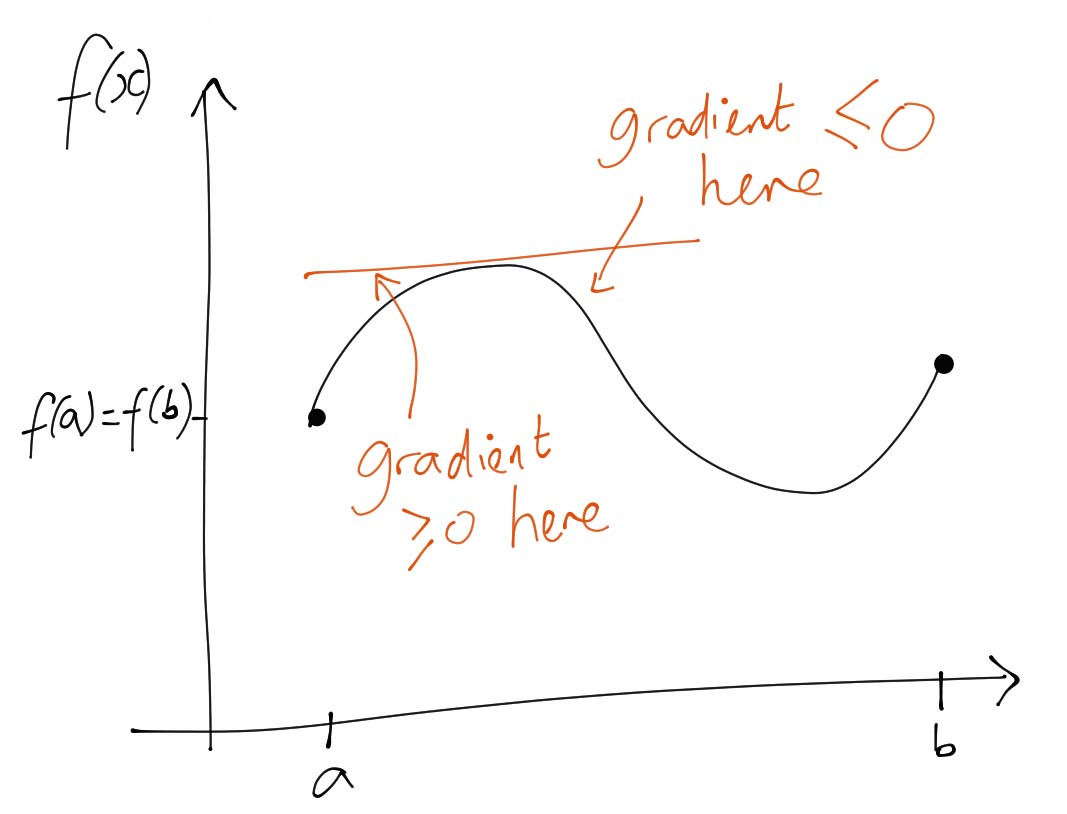
\includegraphics[width = 8cm]{rolle.jpg}
\end{center}


\begin{proof}~
\begin{enumerate}
\item[Case 1.] $f$ is constant on $[a,b]$. Then set $c = \frac{a+b}{2},$ so $f'(c) = \lim_{x\to c}\frac{f(x) - f(c)}{x-c} = 0$.
\item[Case 2.] $f$ takes values $< f(a)$. Then replace $f$ by $-f$ and consider Case 3.
\item[Case 3.] $f$ takes values $> f(a)$. Therefore sup $\{f(x): x \in [a,b]\} > f(a)$ by EVT is realised by some $c \in (a,b)$. Now $f'(c) = \lim_{x\to c} \frac{f(x) - f(c)}{x-c}$. Consider
 \[x > c,~f(x) \leq f(c) \implies \frac{f(x) - f(c)}{x-c} \leq 0 \implies \lim_{x \to c^{+}} \frac{f(x) - f(c)}{x-c} \leq 0\]
 \[x < c,~f(x) \leq f(c) \implies \frac{f(x) - f(c)}{x-c} \geq 0 \implies \lim_{x \to c^{-}} \frac{f(x) - f(c)}{x-c} \geq 0 \] 
 Hence  $\dfrac{f(x) - f(c)}{x-c} = 0$.\qedhere 
\end{enumerate}
	
\end{proof}
\pagebreak

\subsektion{Mean Value Theorem}\vspace*{5pt}


\begin{theorem}[Mean Value Theorem]
If $f:[a,b] \to \RR$ is cts on $[a,b]$ and differentiable on $(a,b)$, then $\exists c \in (a,b)$ such that $f'(c) = \dfrac{f(b) - f(a)}{b-a}$.
\end{theorem}


\begin{center}
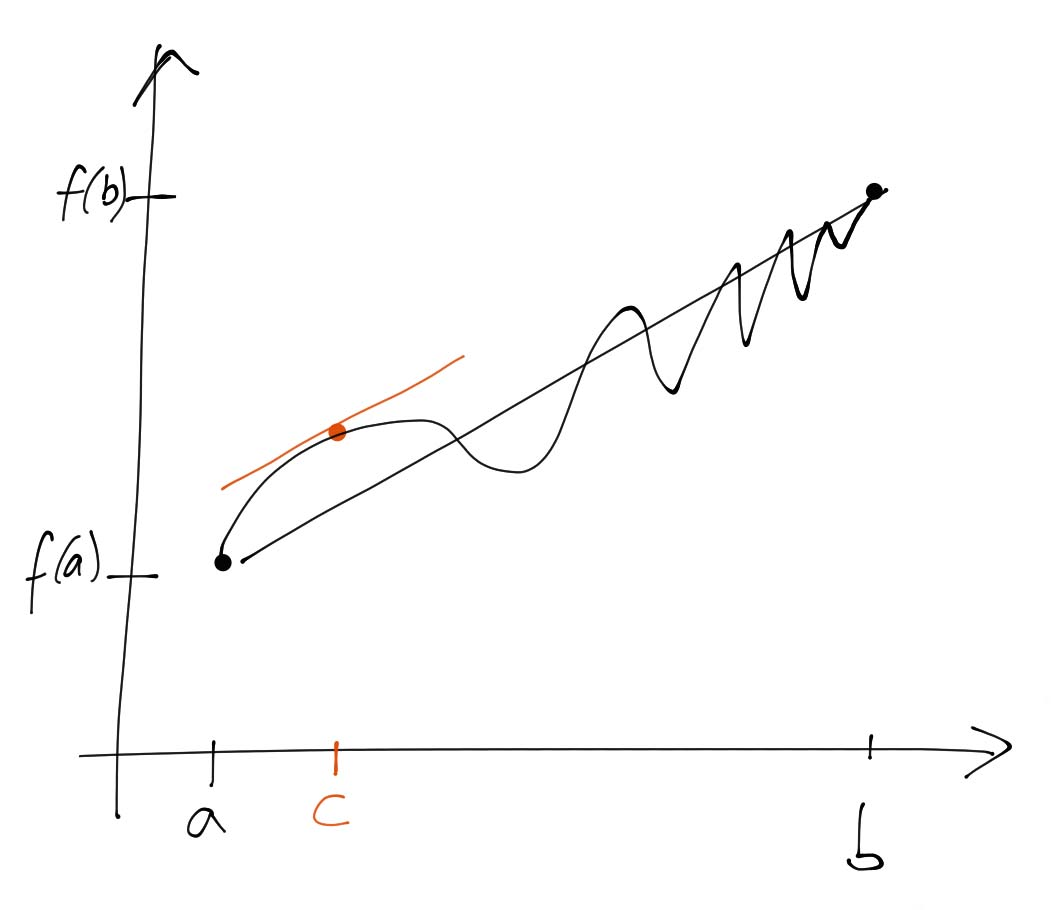
\includegraphics[width = 9cm]{mvt1.jpg}
\end{center}
Note: we can write this as $f(b) = f(a) + (b-a)f'(c)$, $c \in (a,b)$. Compare this to Taylor's Theorem - we're taking just the first $2$ terms of.

\emph{Idea of Proof:} Turn MVT into Rolle. 

\begin{center}
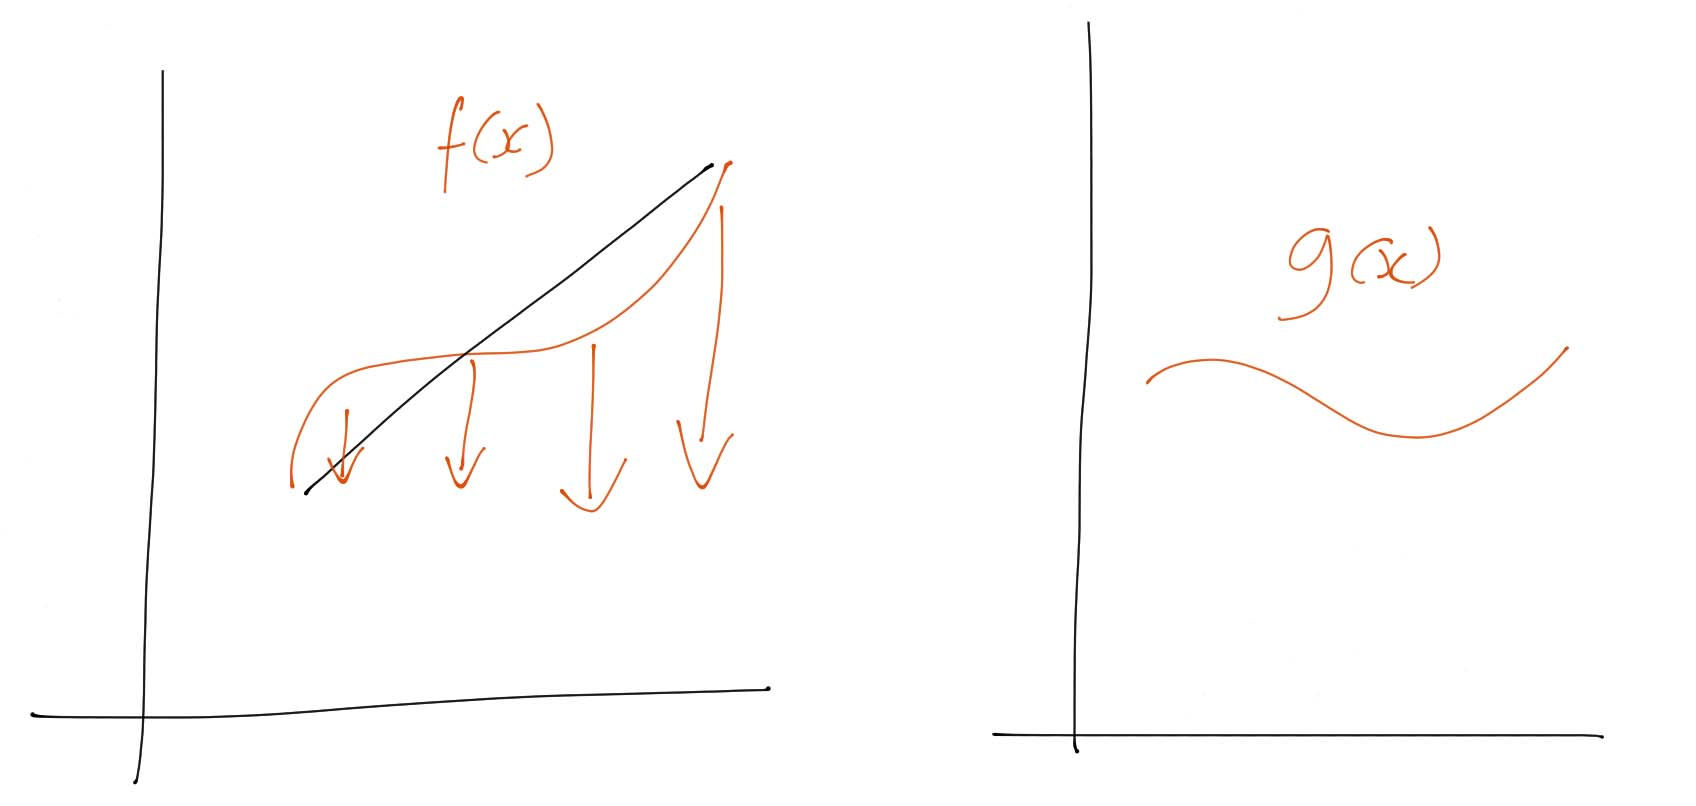
\includegraphics[width = 12cm]{mvt2.jpg}
\end{center}

\begin{proof}
Let $g(x) = f(x) - \dfrac{f(b) - f(a)}{b-a}(x-a)$, which is cts on $[a,b]$ and diff'ble on $(a,b)$. $g(a) = f(a) = g(b)$. By Rolle's Theorem applied to $g$
\[\exists c \in (a,b)\text{ such that }g'(c) = 0 \implies g'(c) = f'(c) - \dfrac{f(b) - f(a)}{b-a}.\qedhere\]	
\end{proof}\vspace*{5pt}

\begin{corollary}
If $f'(x) = 0~\forall x \in (a,b)$. Then $f$ is a constant: $f(x) = f(a)~\forall x \in [a,b]$
\end{corollary}
\begin{proof}
Suppose for a contradiction that $\exists d \in[a,b]$ s.t. $f(d) \neq f(a)$. Then by MVT applied to $\left. f\right|_{[a,d]}: [a,d] \to \RR$, $\exists c\in(a,d)$ s.t. $f'(c) = \dfrac{f(d) - f(a)}{d-a} \neq 0,~\cont$	
\end{proof}


\begin{theorem}[Chain Rule]\lecturemarker{28}{19 March} $g: \RR \to \RR$ diff'ble at $a \in \RR$, $f: \RR \to \RR$ diff'ble at $g(a) \in \RR$, then $f \circ g$ diff'ble at $a$ with $(f\circ g)'(a) =f'(g(a))g'(a)$
\end{theorem}

i.e. \[\left.\frac{d}{dx} f(g(x))\right|_{x=a} = \frac{df}{dx} (g(a)) \frac{dg}{dx}(a) = \left.\frac{df}{dy}\right|_{y=g(a)}\frac{dg}{dx}(a) ``=" \frac{df}{dg}\frac{dg}{dx}\]

\emph{Idea of proof:} 
\[\frac{f(g(x))-f(g(a))}{x-a} = \frac{f(g(x)) - f(g(a))}{g(x) -g(a)}\cdot\frac{g(x)-g(a)}{x-a} \to f'(g(a))\cdot g'(a)\]
problem with this is that $g(x) - g(a)$ might be zero

$\left(\dfrac{h(x) - h(a)}{x-a} \text{ is not defined at } x=a \text{, so define it to be } h'(a) \text{ at } x=a \right)$\\

\begin{proof}
Define $F(g) = \begin{cases}
 	\dfrac{f(y)-f(b)}{g-b} & y \neq b\\
 	f'(g) &  y = b 
 \end{cases}~(\ddagger)$
 where $b = g(a)$. \vspace*{5pt}\\$f$ is diff'ble at $b \implies \lim_{y \to b} F(y) \to f'(b) = F(b)$ as $y \to b$. So $F$ is cts at $b = g(a) ~(*)$. 
 
 $g$ is diff'ble at $a \implies$ cts at $a$. 
 
 By $(*) \implies F \circ g$ is cts at $a \implies F(g(x)) \to F(g(a)) = f'(b)$ as $x \to a ~(**)$. 
 
 So now we can follow the rough proof to write 
 \[\frac{f(g(x)) -f(g(a))}{x} = F(g(x))\frac{g(x) - g(a)}{x-a}\]
 

 
 Now take $\lim_{x\to a}$ to get $(f\circ g)'(a)$ exists and equals $f'(b)g'(a)$ by $(**)$ \end{proof}\vspace*{5pt}
 
 Ex: ``Sum Rule" $f, g$ are differentiable at $a\implies f+g$ are differentiable at $a$ with $(f+g)'(a) = f'(a) + g'(a)$. Pre-ex: Algebra of limit for $\lim_{x\to a}$ is on Question Sheet.\\
 
 \emph{Rough:} $f: \RR\to \RR$ is differentiable and bijective, $g = f^{-1}: \RR \to \RR$.
 
  Suppose $g$ is differentiable. Then by the chain rule $f\circ g(y) = y \implies f'(g(y_0))g'(y_0) = 1~\forall y_0 \implies g'(y) = \frac{1}{f'(g(y))}$. 
  
  Suggests that if $f' \neq 0$, then $g$ is differentiable with derivative $\frac{1}{f'\circ g}$\vspace*{5pt}

\begin{theorem}
	If $f:\RR \to \RR$ is differentiable at $a\in \RR$ with $f'(a) \neq 0$ and $f$ is bijective with inverse $g = f^{-1}$, then $g$ is differentiable at $b = f(a)$ with $g'(b) = \dfrac{1}{f'(g(b))} = \dfrac{1}{f'(a)}.$
\end{theorem}
\begin{proof}
\textit{Lemma:} $f'(a) \neq 0 \implies \exists \delta > 0$ such that $f(x) \neq f(a)$ for $x \in (a-\delta,a + \delta)\backslash\{0\}$.  (Proof is left as exercise - use $\lim_{x\to a}$ definition of $f'$ and MVT) \\

 So $\dfrac{g(y)-g(b)}{y-b} = \dfrac{x-a}{f(x) - f(a)} = 1/\dfrac{f(x)-f(a)}{x-a}$ where $x = g(y),~y \neq b$.
 
 As $y \to b$, $g(y) \to g(b) = a$ since $f$ differentiable at $a \implies f$ cts at $a \implies g$ cts at $b \implies x \to a \implies$ RHS $\to \dfrac{1}{f'(a)}$.	
\end{proof}\vspace*{15pt}



\textbf{Felina.} Suppose $f: \RR \to \RR$ satisfies
\begin{itemize}
\item $f(x) + f(y) = f(x+y)~\forall x,y\iR$
\item $f$ is continuous everywhere	
\end{itemize}

\emph{What if $f$?}

Observe $y = 0: f(x) + f(0) = f(x),~\forall x$, so $f(0) = 0$. 

For $y = 1: f(x) + f(1) = f(x+1)$

\[\begin{aligned}\text{Induction } f(x+2) &= f(x) + f(1) + f(1) \\
f(x+3) &= f(x) + 3f(1)\\
&\vdots \\ 
 f(x+n) &= f(x) + nf(1)\\
\implies f(n) &= nf(1) ~(*)\end{aligned}
\]

Similar mucking about should convince you that $f(x) = xf(1)$. We've proved that for $x\iN$ by $(*)$. $f(1)$ is an unknown constant $c$. [Notice $f(x) = cx$ indeed satisfies the given assumptions]

Notice \lecturemarker{29}{20 March} that $(*)$ holds for $n \iZ$ too
\[f(-n) + f(n) = f(n-n) = f(0) = 0\]
\[\implies f(-n) = -f(n) = -nf(1) = -nc,\quad n \iN\]
$(*)$ also holds for $\QQ$
\[\textstyle{\underbrace{\textstyle{f(\frac{n}{m}) + \dots + f(\frac{n}{m})}}_{m \text{ copies}} = f(\frac{n}{m} + \dots + \frac{n}{m}) =f(n) = cn}\]
\[\textstyle{\implies f(\frac{n}{m}) = c\frac{n}{m} \quad \forall \frac{n}{m} \iQ,~n,n\iZ}\]

\textbf{Claim:} $f(x) = cx$ [$c = f(1)$] $\forall x \iQ$

\emph{Idea:} now is if $x \iR$ then $x$ is close to $y \iQ$. $f$ is continuous $\implies f(x)$ is close to $f(y) = cy$, close to $cx$. So $f(x)$ is arbitrarily ($\forall \epsilon!$) close to $cx \implies f(x) = cx$

(or we could use some machinery to say $\forall x \iR$, $\exists (y_n) \to x$, $y_n \iQ$. Then $f$ is continuous $\implies f(y_n) = cy_n \to f(x)$ and $cy_n \to cx$. So uniqueness of limits $\implies f(x) = cx$.) 

\begin{proof}
Fix $x \iR$. Fix $\epsilon >0$. M1F: $\exists y \iQ$ s.t. $|y-x| < \epsilon \implies |cy - cx| < \epsilon/2$
\[\exists \delta >0\text{ s.t. }|x-y| < \delta \implies |f(x) - f(y)| < \epsilon/2\]

and by M1F again $\exists y\iQ$ s.t. $|y-x| < \mathrm{min}\{\delta,\epsilon/2\}$. 

So $|cy-cx|< \epsilon/2$ and $|f(x) - \equalto{f(y)}{cy}| < \epsilon/2 \implies |f(x) - cx| < 2\epsilon/2 = \epsilon$. 

This is true $\forall \epsilon >0 \implies |f(x) -cx| = 0$
\end{proof}



  \begin{center}
  \textsf{\textbf{- End of Analysis I -}}	
  \end{center}
  
  \stepcounter{lecture}
\setcounter{lecture}{1}

  		% Differentiation


\end{document}